\begin{frame}
    \titlepage
\end{frame}

\setcounter{tocdepth}{1} % Tiefe von Inhaltsverzeichnis
\begin{frame}
    \tableofcontents
\end{frame}

\section{Aufgabenstellung und Produktanforderungen} % Peter
\subsection{Aufgabenstellung}
\section{Aufgabenstellung und Produktanforderungen} % Peter
\subsection{Aufgabenstellung}
\begin{frame}
    \frametitle{Aufgabenstellung}
	\begin{block}{Aufgabenstellung}
	    \begin{itemize}
	    	\item 5 Tennisbälle
	    	\item 1 Korb
		    \item 1 Spielfeld
		    \item 1 Ziel!
	    \end{itemize}
    \end{block}
\end{frame}

\section{Realisierung}
%\begin{frame}
%    \frametitle{Übersicht}
%    \begin{columns}
%        \begin{column}{0.50\textwidth}
%            \centering
%            \includegraphics[width=1.00\textwidth]{../doc/fig/Bild_mit_Kamera.png}
%        \end{column}
%        \begin{column}{0.50\textwidth}
%            \begin{block}{Komponenten}
%                \begin{itemize}
%                    \item Kamera
%                    \item Drehvorrichtung
%                    \item Turm
%                    \item Balllager
%                    \item Ballnachschub
%                    \item BLDC Motor
%                \end{itemize}
%            \end{block}
%        \end{column}
%    \end{columns}
%\end{frame}
\begin{frame}
    \frametitle{Übersicht}
    \begin{columns}
        \begin{column}{1.00\textwidth}
            \begin{figure}[h]
                \centering
                \begin{tikzpicture}[scale=1.00]
                    \node[above right] (img) at (0,0) {\includegraphics[width=0.50\textwidth]{../doc/fig/Bild_mit_Kamera.png}};
                    \draw[line width=1pt]
                        (0, 4) node[left=0mm] {Balllager}
                        -- (1.5, 3.7);
                    \fill (1.5, 3.7) circle (2pt);
                    \draw[line width=1pt]
                        (1, 5) node[left=0mm] {Ballnachschub}
                        -- (2.5, 4.7);
                    \fill (2.5, 4.7) circle (2pt);
                    \draw[line width=1pt]
                        (6.0, 3.0) node[right=0mm] {Drehvorrichtung}
                        -- (3.0, 2.4);
                    \fill (3.0, 2.4) circle (2pt);
                    \draw[line width=1pt]
                        (5.0, 6.0) node[right=0mm] {BLDC Motor}
                        -- (3.2, 6.0);
                    \fill (3.2, 6.0) circle (2pt);
                    \draw[line width=1pt]
                        (5.5, 4.5) node[right=0mm] {Turm}
                        -- (3.5, 3.5);
                    \fill (3.5, 3.5) circle (2pt);
                    \draw[line width=1pt]
                        (6.5, 1.5) node[right=0mm] {Kamera}
                        -- (3.7, 2.0);
                    \fill (3.7, 2.0) circle (2pt);
                \end{tikzpicture}
            \end{figure}
        \end{column}
    \end{columns}
\end{frame}


\section{Übersicht Maschinentechnik}

\subsection{Beschreibung der Komponenten}

Die Konstruktion besteht hauptsächlich aus Aluminium-Blechteilen. Einige 
Komponenten müssen aus konstruktiven Gründen als Frästeile ausgeführt werden. 
Um ein geringeres Gewicht zu erreichen, werden die Blechteile mit Aussparungen 
an nicht erforderlichen Flächen versehen. Da dies eine Schwächung der 
Stabilität mit sich bringt, werden die Aussparungen, wie im Flugzeugbau 
üblich, mit gebogenen Innenkanten ausgeführt.

\begin{figure}[h!]          
    \centering             
    \includegraphics[width=0.5\textwidth]{fig/IMAG0364.jpg}
    \caption{Seitenteil Balllager}
    \label{fig:Seitenteil Balllager}        
\end{figure}

\subsubsection{Balllager}
Das Balllager dient als Grundstruktur, an welcher der Ballnachschub und der 
Motor befestigt sind. Gelagert werden die Bälle im Inneren des quadratischen 
Querschnittes. Die Halterungen des Motors werden jeweils auf beiden 
Aussenseiten des vorderen Endes befestigt. Damit das Stahlband des 
Ballnachschubs optimal aufgewickelt werden kann, werden die herausstehenden 
Enden der Nieten mit Aluminiumleisten abgedeckt. Diese können gleichzeitig als 
Kabelkanal verwendet werden. 

\begin{figure}[h!]          
    \centering             
    %\includegraphics[width=0.5\textwidth]{fig/balllager.jpg}
    \caption{jfdslj}
    \label{fig:hhjfdhfd}        
\end{figure}

\subsubsection{Ballnachschub}
Der Ballnachschub besteht im Wesentlichen aus einer Trommel, einem Stahlband 
und einem Servomotor. Das Stahlband wird im Inneren des Balllagers um die 
Bälle herum ausgelegt. Durch das Aufwickeln des Bandes auf die Trommel werden 
die Bälle Richtung Beschleunigungsrad gezogen. Der Antrieb erfolgt durch einen 
umgebauten Servomotor, welcher mittels Zahnriemen mit der Welle der Trommel 
verbunden ist.

\begin{figure}[h!]          
    \centering             
    %\includegraphics[width=0.5\textwidth]{fig/ballnachschub.jpg}
    \caption{jfdslj}
    \label{fig:hhjfdhfd}        
\end{figure}

\paragraph{Auslegung}
Als Servo dient ein HS85MG der Firma Hitec. Dieses ist wie folgt spezifiziert: 
\begin{table}[h!]
    \centering
    \begin{zebratabular}{lll}
        \rowcolor{gray}
        Parameter &
        Wert bei 4.8\si{\volt} &
        Wert bei 6.0\si{\volt} \\
        Stellgeschwindigkeit (60\si{\degree}) &
        0.16\si{\second} &
        0.14\si{\second} \\
        Drehmoment &
        3.0\si{\kilogram\per\centi\metre} &
        3.5\si{\kilogram\per\centi\metre} \\
    \end{zebratabular}
    \caption{Spezifikation Servomotor}
\end{table}
Dies ergibt folgende Spezifikationen für den sich daraus ergebenden DC Motor: 
\begin{table}[h!]
    \centering
    \begin{zebratabular}{lll}
        \rowcolor{gray}
        Parameter &
        Wert bei 4.8\si{\volt} &
        Wert bei 6.0\si{\volt} \\
        Stellgeschwindigkeit (60\si{\degree}) &
        62.5\si{\per\minute} &
        71.4\si{\per\minute} \\
        Drehmoment &
        0.3\si{\newton\metre} &
        0.35\si{\newton\metre} \\
    \end{zebratabular}
    \caption{Spezifikation DC Motor}
\end{table}
Beim Dauerbetrieb zeigt sich dieser Motor als zu schwach. Um eine akzeptable 
Abschusskadenz zu erreichen muss er mit einer Spannung von 16\si{\volt} 
betrieben werden. Dieser Belastung ist der Motor nicht gewachsen. Nach einigen 
Versuchen weist er einen Kurzschluss auf und muss ersetzt werden. Als Ersatz 
kommt ein Servo vom Typ ??? von Conrad zum Einsatz. 

\subsubsection{Drehvorrichtung}
Die Drehvorrichtung dient zur horizontalen Ausrichtung der 
Abschussvorrichtung. Um eine genaue Positionierung und ausreichende Stabilität 
zu ermöglichen, wurde ein Zahnrad durch zwei Axial-Rillenkugellager auf einer 
Grundplatte verspannt. Die Ausrichtung wird durch einen Schrittmotor mit dem 
direkt verbundenen, kleineren Zahnrad eingestellt. Einen guten Bodenkontakt 
garantieren an der Unterseite der Füsse angeklebte Gummimatten.

\begin{figure}[h!]          
    \centering             
    %\includegraphics[width=0.5\textwidth]{fig/drehvorrichtung.jpg}
    \caption{jfdslj}
    \label{fig:hhjfdhfd}        
\end{figure}

\paragraph{Auflösung}
Der Schrittmotor benötigt 200 Schritte für eine Umdrehung. Er wird mit 1/128 
Mikrosteps angesteuert. Die Übersetzung beträgt 1:4.8. Daraus ergibt sich 
folgende Auflösung: 
\[ 200 \cdot 128 \cdot 4.8 = 122'880 \frac{\text{Schritte}}{\text{Umdrehung}}  \]
\[ \frac{360^\circ}{122'880} = 0.0029296875 \frac{^\circ}{\text{Schritt}} 
= 0.17578 \frac{'}{\text{Schritt}} = 10.547 \frac{''}{\text{Schritt}}
\rightarrow 341.33 \frac{\text{Schritte}}{^\circ}\]

\subsubsection{Motor}
Der Motor für die Ballbeschleunigung wird als Eigenkonstruktion ausgeführt.  
Der Läufer dient dabei als Felge des Beschleunigungsrades und wird aus 
Aluminium gefräst. Als Grundlage für den Motor dienen Motoren aus 
Diskettenlaufwerken. Diese besitzen 10 Polpaare und 15 Nuten. Diese 
Konfiguration wird grundsätzlich beibehalten. Jedoch wird der neue Motor aus 
den Statorblechen von zwei Diskettenlaufwerkmotoren aufgebaut. Dies dient 
dazu, den magnetischen Querschnitt zu vergrössern. Für die Dauermagnete des 
Rotors kam im Laufwerk ein Magnetring zum Einsatz. Im neuen Rotor werden die 
Dauermagnete mittels Neodymmagneten realisiert. Dabei wird ein Halbach-Array 
aufgebaut. Deshalb kommen Magnete mit einer quadratischen Grundfläche zum 
Einsatz. 
\begin{figure}[h!]
    \centering
    \includegraphics[width=0.5\textwidth]{fig/halbach.pdf}
    \caption{Ausschnitt aus verwendetem Halbach-Array mit Rückschlussring}
    \label{fig:halbach}
\end{figure}
Ein Halbach-Array hat den Vorteil, dass die Feldlinien auf einer 
Seite gebündelt werden, sich auf der Anderen hingegen beinahe aufheben. 
Als Rückschluss kommt ein Stahlring zum Einsatz, welcher in den Rotor 
eingepresst wird. Dieser dient dazu, die Magnetfeldlinien hinter den 
Dauermagneten zu bündeln und so den magnetischen Kreis zu schliessen. 

\begin{figure}[h!]          
    \centering             
    %\includegraphics[width=0.5\textwidth]{fig/motor.jpg}
    \caption{jfdslj}
    \label{fig:hhjfdhfd}        
\end{figure}

\subsubsection{Turm}
Der Turm dient als Verbindungselement des Balllagers mit dem grösseren Zahnrad 
der Drehvorrichtung. Ausgeführt wird die gesamte Konstruktion aus 
Aluminiumblech. Der Platz im Inneren wird zum Verstauen der 
Elektronikkomponenten verwendet, deswegen wird die vordere Abdeckplatte als 
Wartungsklappe ausgeführt. Die Abdeckplatte wird mit Schrauben anstatt mit 
Nieten befestigt.

\begin{figure}[h!]          
    \centering             
    %\includegraphics[width=0.5\textwidth]{fig/turm.jpg}
    \caption{jfdslj}
    \label{fig:hhjfdhfd}        
\end{figure}

\clearpage

%\subsection{Herstellung mechanische Komponenten}
Die konzeptionellen CAD-Zeichnungen werden ab Semesterwoche 2 weiter 
ausgearbeitet, abgewickelt und die Fertigungszeichnungen erstellt. Hierbei 
müssen hauptsächlich Details wie Bohrungen für die Nieten angebracht und 
einige konstruktive Anpassungen vorgenommen werden. 

Ab Semesterwoche 3 können die ersten Teile an der Fräsmaschine im 
Elektrotechniklabor produziert werden, wobei parallel  hierzu die restlichen 
Komponenten am CAD fertiggestellt werden.  Um die gebogenen Innenkanten der 
Aussparungen zu realisieren, werden die gefrästen Blechteile mit einer 
Handpresse und eigens hierfür hergestellten Werkzeugen gefertigt.

In Semesterwoche 4 werden die Grundplatte zur Fertigung an der HSLU in Auftrag 
gegeben.

In Semesterwoche 5 werden zusätzlich einige Teile zum spanenden Herstellen, 
sowie zum 3D-Drucken in Auftrag gegeben. Ebenfalls wird eine 
Rohmaterialbestellung abgegeben.

Die in Auftrag gegebenen Teile können in Semesterwoche 6 abgeholt werden, 
wobei das  Rohmaterial fälschlicherweise aus Stahl, anstatt aus Aluminium, 
bestellt wurde. Eine neue Bestellung des richtigen Rohmaterials wurde abgesetzt.

In Semesterwoche 7 können die bestellten Teile sowie die zum biegen extern in 
Auftrag gegebenen Teile abgeholt werden. Des weiteren wird mit dem Zusammenbau 
der einzelnen Komponenten begonnen. Aufgrund eines beim Biegen entstandenen 
Verzugs einzelner Bauteile und einiger konstruktiver Ungenauigkeiten müssen 
diverse Bohrungen durch feilen nachgebessert werden. Durch Niethefter kann die 
Konstruktion bis zum endgültigen Vernieten aufgebaut werden.

\begin{figure}[h!]          
	\centering             
	\includegraphics[width=0.5\textwidth]{fig/IMG_2290.JPG}
	\caption{Zusammenbau Balllager}
	\label{fig:Zusammenbau Balllager}        
\end{figure}

\begin{figure}[h!]          
	\centering             
	\includegraphics[width=0.5\textwidth]{fig/IMG_2303.JPG}
	\caption{Unvollständiger Aufbau}
	\label{fig:Unvollständiger Aufbau}        
\end{figure}

\paragraph{Nachfolgend werden die speziellen Anpassungen einzelner Komponenten genauer beschrieben:}

\paragraph{Balllager}
Anhand der Erfahrungen erster Testläufe wird entschieden, keine Verstärkung an 
der Unterseite des vorderen Endes anzubringen. Diese Verstärkung hätte eine zu 
starke Durchbiegung des Blechs beim Abschuss der Bälle verhindert.

\paragraph{Ballnachschub}
Beim Zusammenbau wird festgestellt, dass die Welle der Trommel einen zu 
grossen Durchmesser hat und daher mit Hilfe einer Handbohrmaschine und 
gewöhnlichem Schleifpapier auf das gewünschte Mass geschliffen werden muss.

\paragraph{Drehvorrichtung}
Um weiteres Gewicht einzusparen wird die bereits hergestellte Grundplatte auf die halbe Höhe überfräst.

\begin{figure}[h!]          
	\centering             
	\includegraphics[width=0.5\textwidth]{fig/IMAG0357.jpg}
	\caption{Überfräsen der Grundplatte}
	\label{fig:Grundplatte fräsen}        
\end{figure}

\paragraph{Motor}
Zunächst wird der Rotor des Motors auf einer CNC-Fräse gefräst und der 
Stahlring eingepresst. Anschliessend werden sämtliche Magnete von Hand 
eingesetzt und mit Zweikomponentenklebstoff befestigt. Die Statorbleche für 
den Motor stammen aus Floppydisk-Laufwerken. Dazu müssen für einen Motor die 
Statoren aus zwei Laufwerken ausgebaut werden. Anschliessend werden die 
bestehenden Wicklungen von den Statoren entfernt. Die Statorbleche und die 
Kunststoffisolatoren werden für den neuen Motor weiterverwendet. Dazu werden 
die Statorbleche aus zwei Motoren aufeinandergelegt und mit der Halterung 
verschraubt. Anschliessend wird der Stator mit neuem Kupferlackdraht 
bewickelt. Nach dem Bewickeln und fixieren der Wicklungen wird der Stator 
passend auf den Durchmesser des Rotors abgedreht. Danach kann der Stator auf 
der passenden Aufnahme befestigt und der Motor zusammengesetzt werden. 
\begin{center}
    \begin{minipage}[c]{0.2\textwidth}
        Bild Floppy (2759)
    \end{minipage}
    \begin{minipage}[c]{0.1\textwidth}
        \Huge$\Rightarrow$
    \end{minipage}
    \begin{minipage}[c]{0.2\textwidth}
        Stator leer (???)
    \end{minipage}
    \begin{minipage}[c]{0.1\textwidth}
        \Huge$\Rightarrow$
    \end{minipage}
    \begin{minipage}[c]{0.2\textwidth}
        Stator bewickelt (2816 / 2751)
    \end{minipage}
\end{center}

Beim Zusammenbau wird bemerkt, dass die Langlöcher der Motorenhalterung zu kurz ausgeführt wurden um einen guten Anpressdruck der Bälle zu ermöglichen. Daher werden diese durch feilen verlängert.

\paragraph{Turm}
Die Muttern der Wartungsklappe werden auf der Innenseite des Turms mit Zweikomponentenklebstoff 
angebracht. 

\begin{figure}[h!]          
	\centering             
	\includegraphics[width=0.3\textwidth]{fig/IMG_2292.JPG}
	\caption{Kleben der Muttern}
	\label{fig:Muttern Kleben}        
\end{figure}



\subsection{Korberkennung}
\begin{frame}
    \frametitle{Grundplatte}
    \begin{columns}
        \begin{column}{0.9\textwidth}
            \centering
            \includegraphics[width=1.0\textwidth]{FotosM/Bild2.jpg}
        \end{column}
    \end{columns}
\end{frame}
\begin{frame}
    \frametitle{Kamera}
    \begin{columns}
        \begin{column}{0.9\textwidth}
            \centering
            \includegraphics[width=1.0\textwidth]{../doc/fig/DSC02993.JPG}
        \end{column}
    \end{columns}
\end{frame}

\begin{frame}
    \frametitle{Korberkennung}
    \framesubtitle{Korberkennung}
    \begin{columns}
        \begin{column}{0.4\textwidth}
            \begin{block}{Korberkennung}
                \begin{itemize}
                    \item Kamera
                    \item OpenCV
                \end{itemize}
            \end{block}
        \end{column}
        \begin{column}{0.6\textwidth}
            \centering
            \includegraphics[width=1.0\textwidth]{../doc/fig/BildMitKorb_markiert.png}
        \end{column}
    \end{columns}
\end{frame}


\input{i_korberkennung_ablauf}
\subsection{Ausrichtung}
\begin{frame}
    \frametitle{Kommunikation}
    \begin{columns}
        \begin{column}{1\textwidth}
            \centering
            \includegraphics[width=1.0\textwidth]{../fig/Klassendiagramm_Bluetoothmodul.png}
        \end{column}
    \end{columns}
\end{frame}


\subsection{Controllplatine}
\label{sec:control}
Als Steuerplatine kommt ein FRDM-KL25Z von Freescale zum Einsatz. 
Darauf wird wird ein FreeRTOS als Betriebssystem eingesetzt. 
Für die Ansteuerung der Peripherie und der externen Komponenten 
werden Komponenten mit Processor Expert erzeugt. 
\begin{figure}[h!]
    \centering
    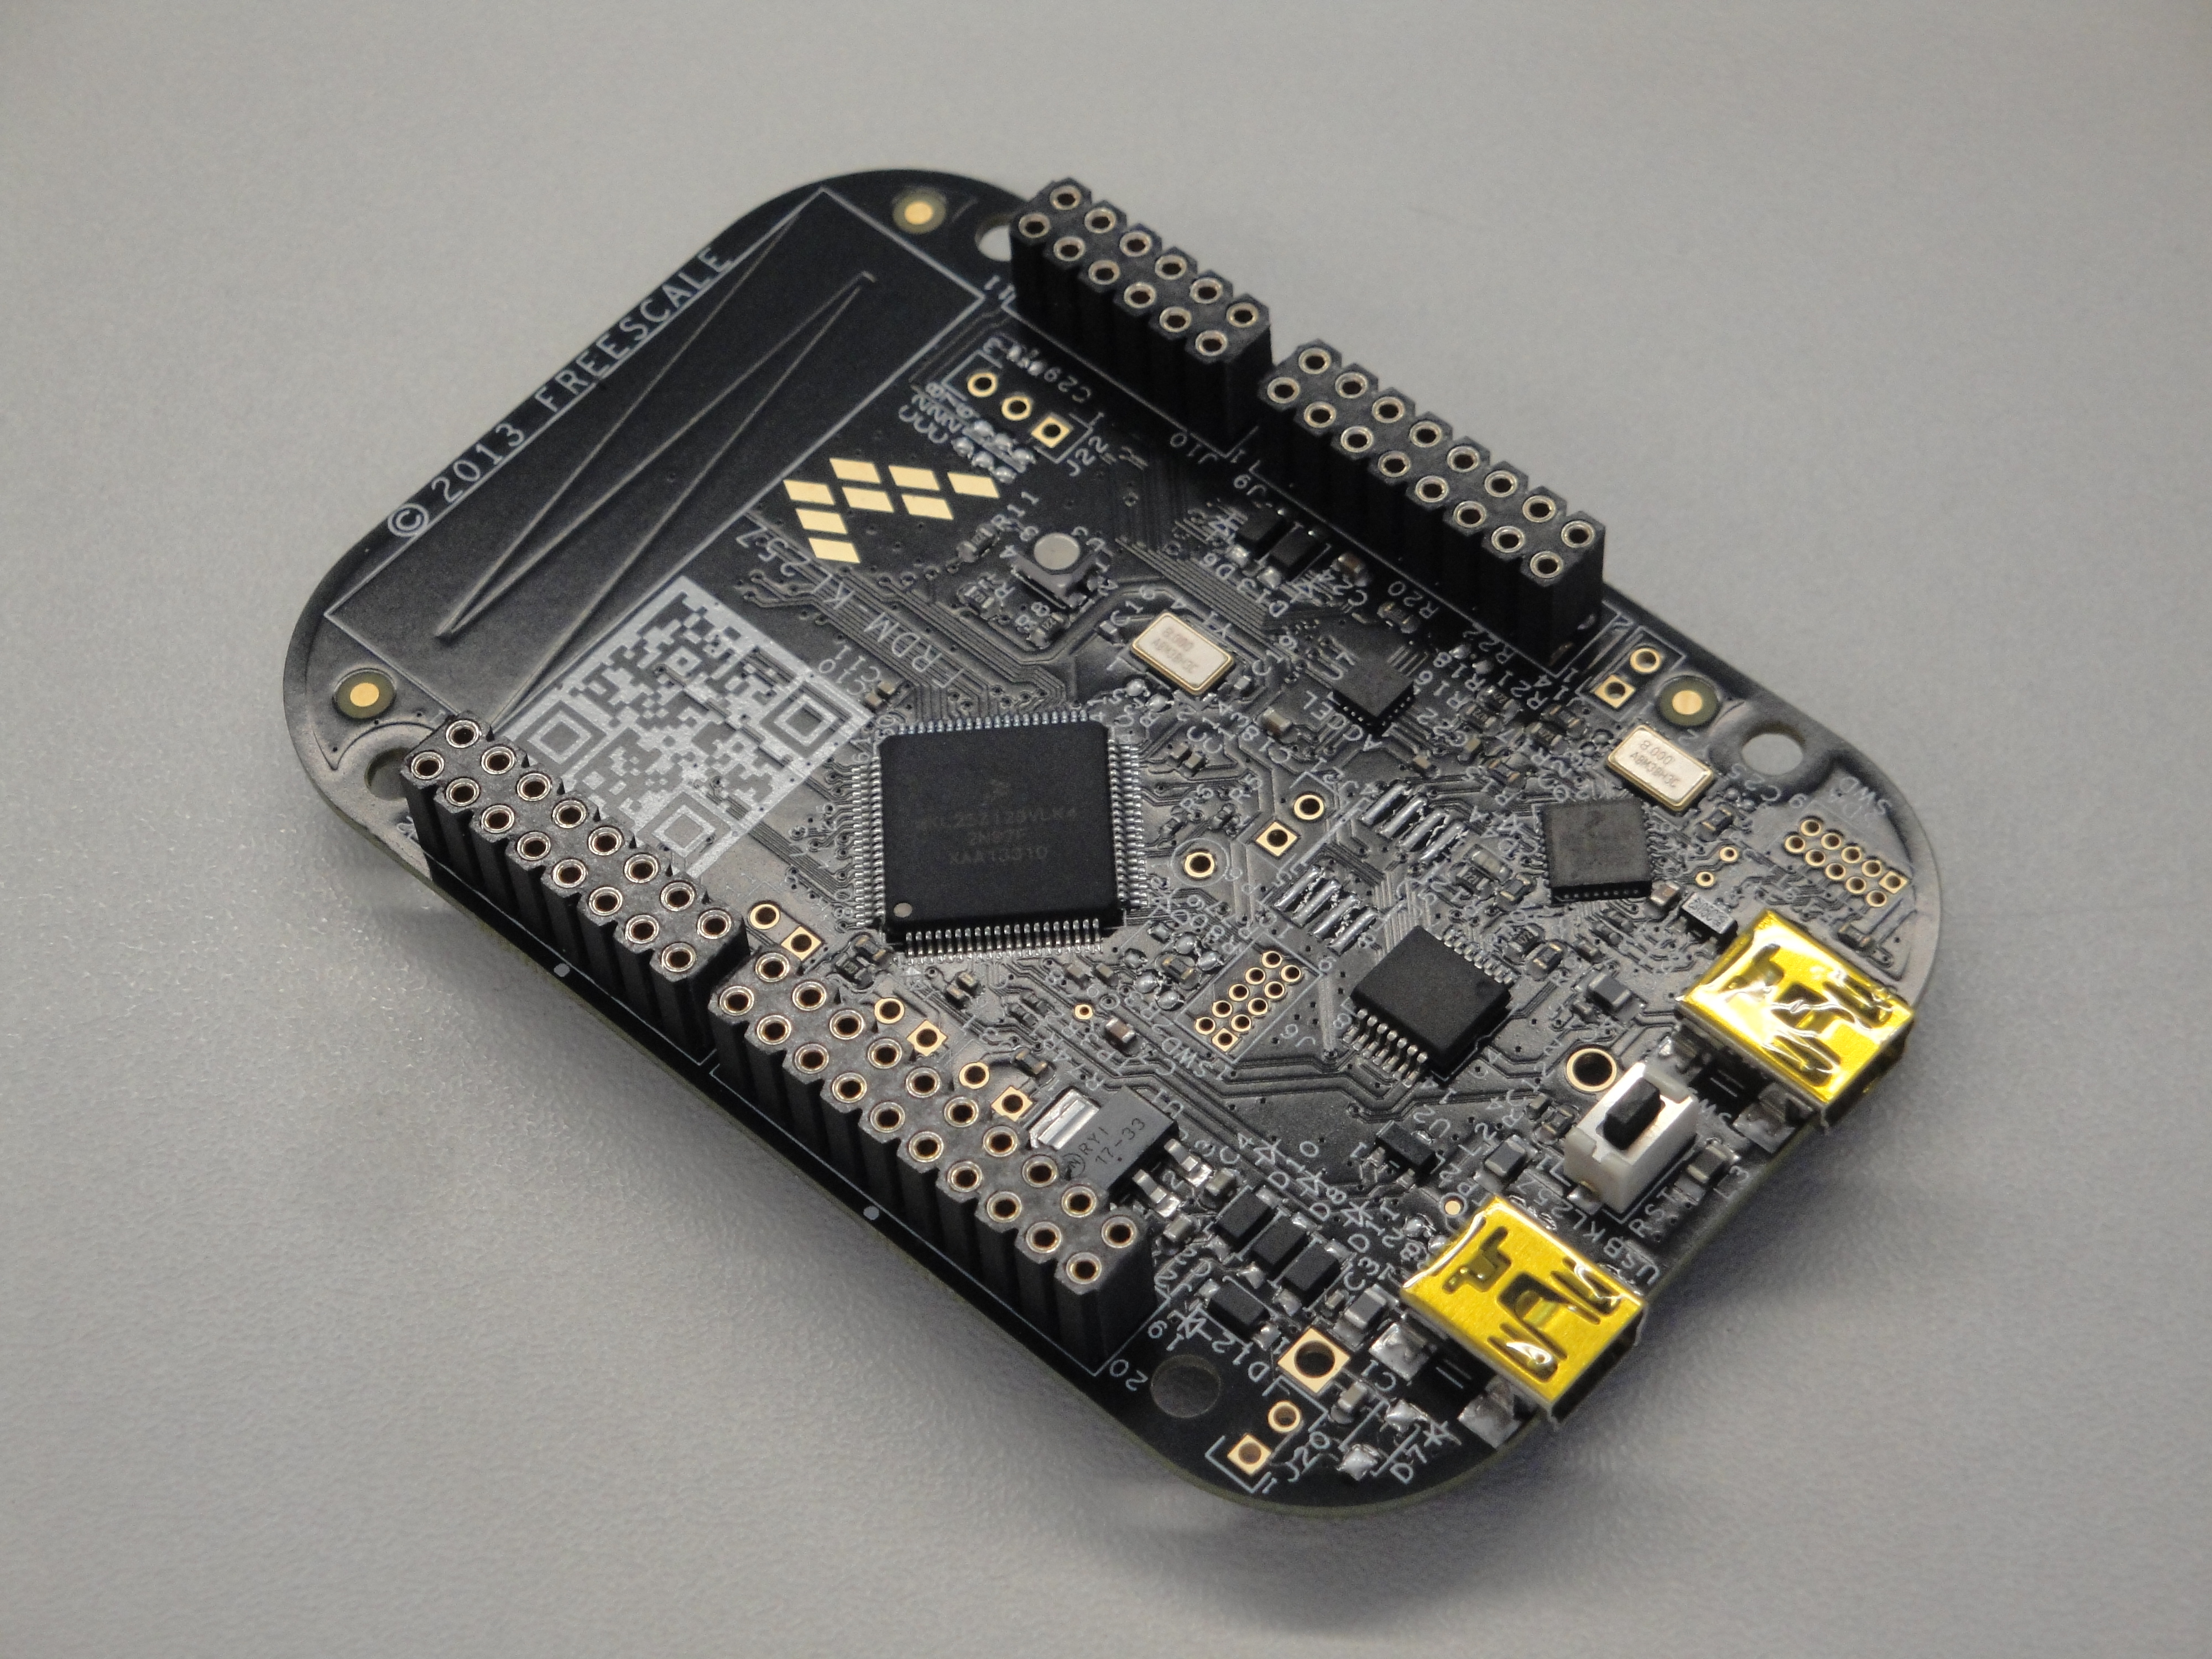
\includegraphics[width=0.45\textwidth]{fig_pcb/DSC02907.JPG}
    \caption{Kontrollplatine - FRDM-KL25Z}
    \label{fig:dc}
\end{figure}

\begin{table}[h!]
    \centering
    \begin{zebratabular}{p{0.21\textwidth}p{0.16\textwidth}p{0.5\textwidth}}
        \rowcolor{gray}
        Name                & Komponente        & Beschreibung \\
        FRTOS1              & FreeRTOS          & Echtzeit-Betriebssystem \\
        Cpu                 & MKL25Z128VLK4     & Controller \\
        UTIL1               & Utility           & Funktionen zur Verarbeitung von Zeichenketten \\
        WAIT1               & Wait              & Delays \\
        CS1                 & CriticalSection   & Deaktivieren von Interrupts für kritische Stellen im Code \\
        AS1                 & AsynchroSerial    & Serielle Schnittstelle via USB $\leftrightarrow$ UART Brücke \\
        TU1                 & TimerUnit\_LDD    & Timer für PWM \\
        TU2                 & TimerUnit\_LDD    & Timer für Timing Ballbeförderung\\
        LedRed              & LED               & Rote LED \\
        Ledgreen            & LED               & Grüne LED \\
        CLS1                & Shell             & Shell \\
        BT1                 & Bluetooth\_EGBT   & Bluetooth Modul \\
        BLDCspi             & SynchroMaster     & SPI zu BLDC Ansteuerung \\
        CS\_BLDC            & BitIO             & Chip Select für BLDC Ansteuerung \\
        BLDC1\_IRQ          & ExtInt            & Interrupt Pin für BLDC Ansteuerung \\
        Stepperspi          & SynchroMaster     & SPI zu Schrittmotor Ansteuerung \\
        STP\_BSY            & ExtInt            & Interrupt für das Signal Busy der Schrittmotor Ansteuerung \\
        PWM1                & PWM               & PWM für DC Motor \\
        DIR                 & BitIO             & Drehrichtung für DC Motor \\
        ENDSW\_SHOOT\_IRQ   & ExtInt            & Interrupt für optionalen oberen Endschalter \\
        ENDSW\_LOAD\_IRQ    & ExtInt            & Interrupt für optionalen unteren Endschalter \\
        HF1                 & HardFault         & Komponente um schwerwiegende Systemfehler debuggen zu können \\
        TI1                 & TimerInt          & Interrupt für Timing Ballbeförderung \\
    \end{zebratabular}
    \caption{Komponenten für das FRDM-KL25Z}
    \label{tab:comp_frdm}
\end{table}

\subsection{Ansteuerung Schrittmotor}
\label{sec:stepperdriver}
Die Ansteuerung für den Schrittmotor wird in der Gruppe PREN-ET entwickelt. 
(Siehe \ref{sec:pren-et} \nameref{sec:pren-et}) 
%Daher werden hier nur Anpassungen für das Team 27 betrachtet. 
\begin{figure}[h!]
    \centering
    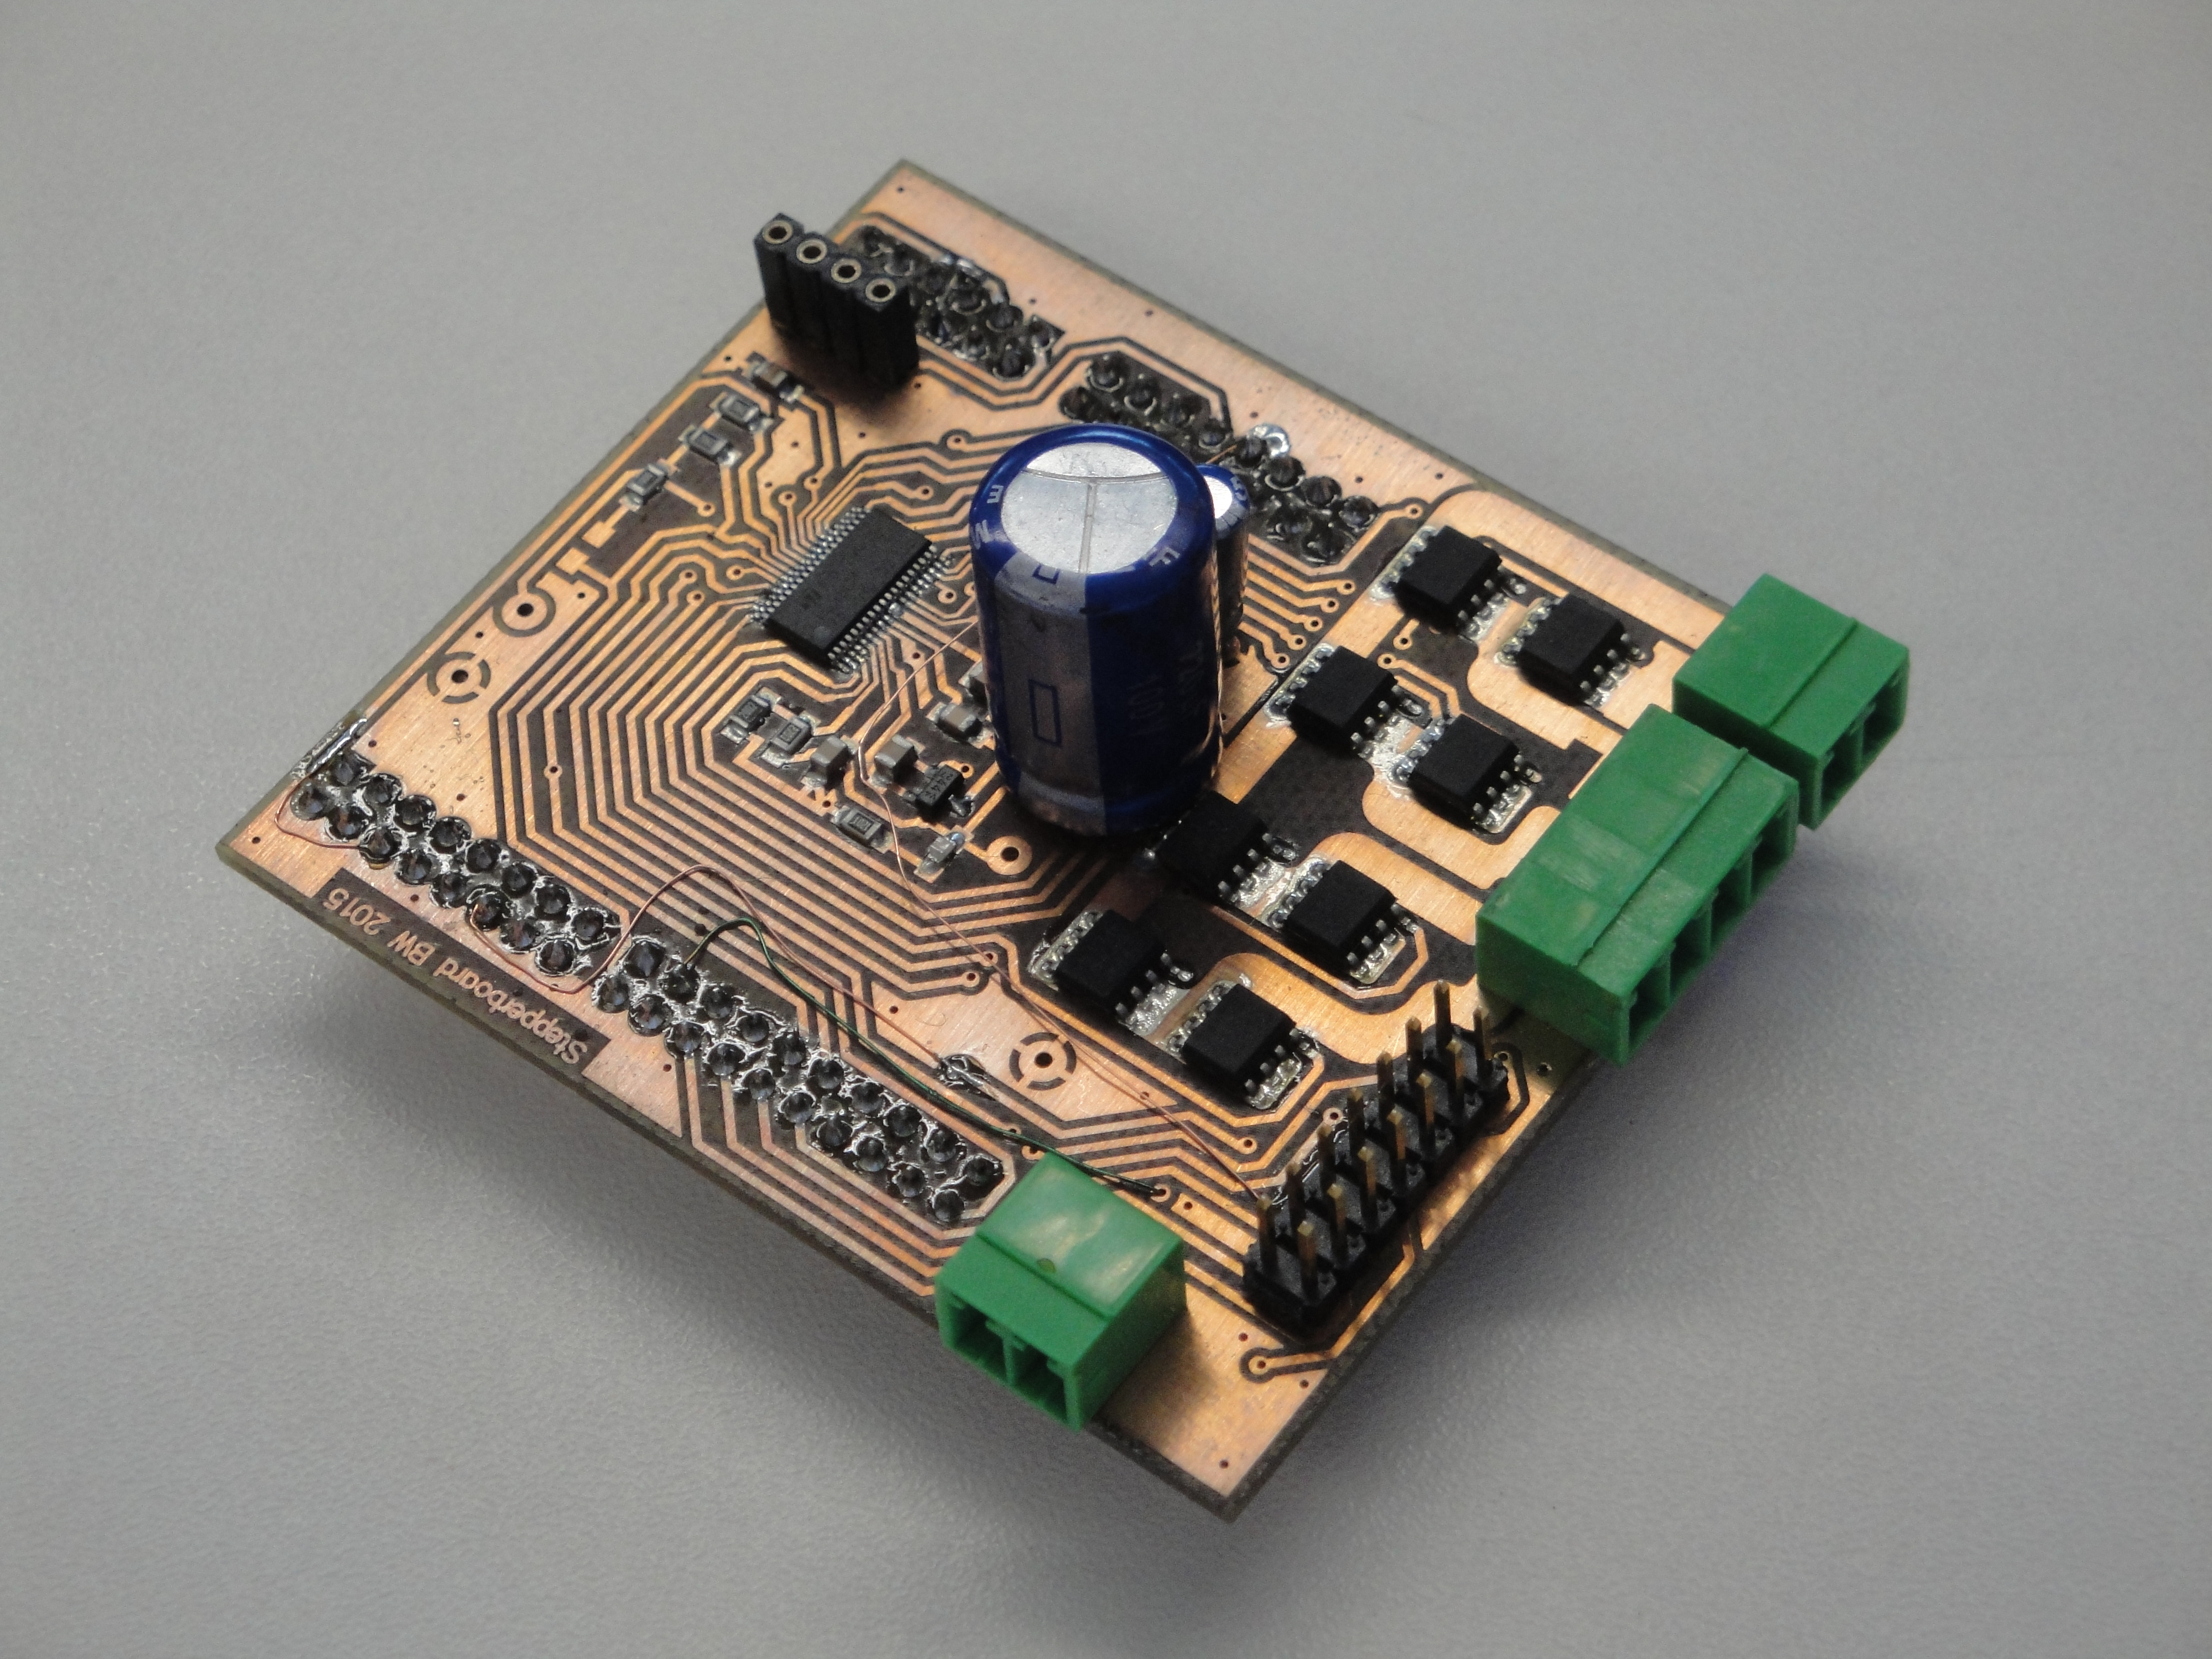
\includegraphics[width=0.7\textwidth]{fig_pcb/DSC02908.JPG}
    \caption{Ansteuerung Schrittmotor}
    \label{fig:dc}
\end{figure}

\noindent
Die Platine mit der Schrittmotoransteuerung kann direkt auf das 
Controllerboard (siehe \ref{sec:control}) gesteckt werden. Die weiteren 
Komponenten können mit einem Flachbandkabel an der Schrittmotoransteuerung 
angeschlossen werden. Das Bluetoothmodul wird direkt auf die 
Schrittmotorsteuerung gesteckt. Es kann ein bipolarer Schrittmotor 
angeschlossen werden. Dieser kann mit einer Auflösung von 1/128 Mikrosteps 
angesteuert werden. 

\subsection{Fachgruppe Elektrotechnik}
\label{sec:pren-et}
Elektrotechnik-Studierenden aus mehreren Gruppen haben sich
zusammengeschlossen um gemeinsame Probleme anzugehen. Dabei handelt es sich
um die benötigte Hard- und Software, um Motoren anzusteuern
und gegebenenfalls zu regeln. In diesem Zusammenschluss werden drei Gruppen
gebildet, um Lösungen für DC-, Stepper- und Brushless-Motoren auszuarbeiten.
Die Idee besteht darin, dass nicht jede Gruppe für dasselbe Problem wo
möglich denselben Lösungsansatz verfolgt, sondern die Ressourcen kombiniert,
Synergien nutzt, um eine bessere Lösung zu erarbeiten. Auf diese Weise kann
das teamübergreifende Arbeiten im Rahmen des PREN erlernt und
geübt werden. Somit wird Idee der Interdisziplinarität im erweiterten Sinn
Rechnung getragen. Die Gruppen und deren Mitglieder sind in 
\autoref{tab:pren-et-members} aufgeführt.
\begin{table}[h!]
    \centering
    \begin{zebratabular}{lllccc}
        \rowcolor{gray} 
        Team & Mitglied         & Github    & DC          & BLDC        & Stepper     \\
        27   & Daniel Winz      & daniw     &             & \textbullet & \textbullet \\
        32   & Yves Studer      & ystuder   &             & \textbullet &             \\
        33   & Flavio Kreiliger & Flavinsky & \textbullet &             & \textbullet \\
        38   & Bettina Wyss     & BettyET   &             &             & \textbullet \\
        39   & Ervin Mazlagi\'c & ninux     & \textbullet &             &             \\
    \end{zebratabular}
    \caption{Übersicht der PREN-ET Projektgruppen}
    \label{tab:pren-et-members}
\end{table}
Für den Austausch und die Ablage von Daten und Unterlagen wird die Plattform 
Github ausgewählt, da damit via Git\footnote{Verteiltes 
Versionskontrollsystem} versioniert werden kann. Dazu wird auf Github die 
Organisation PREN-ET gegründet. Diese ist unter 
\url{https://github.com/PREN-ET} einsehbar. für die einzelnen Projekte werden 
Repositories angelegt. Diese sind in \autoref{tab:pren-et-repos} aufgeführt. 
\begin{table}[h!]
    \centering
    \begin{zebratabular}{p{0.09\textwidth}p{0.37\textwidth}p{0.4\textwidth}}
        \rowcolor{gray} 
        Repository  & Link         & Beschreibung \\
        info        & \url{https://github.com/PREN-ET/info}    & Allgemeine Informationen zur Organisation von PREN-ET \\
        doc         & \url{https://github.com/PREN-ET/doc}     & Dokumentation \\
        dc          & \url{https://github.com/PREN-ET/dc}      & Treiber für Gleichstrommotoren \\
        bldc        & \url{https://github.com/PREN-ET/bldc}    & Treiber für Brushless Motoren \\
        stepper     & \url{https://github.com/PREN-ET/stepper} & Treiber für Schrittmotoren \\
        frdm        & \url{https://github.com/PREN-ET/frdm}    & Beispiele zur Ansteuerung mittels FRDM-KL25Z \\
    \end{zebratabular}
    \caption{Übersicht der PREN-ET Repositories}
    \label{tab:pren-et-repos}
\end{table}

\begin{frame}
    \frametitle{Ausrichtung}
    \begin{columns}
        \begin{column}{0.8\textwidth}
            \centering
            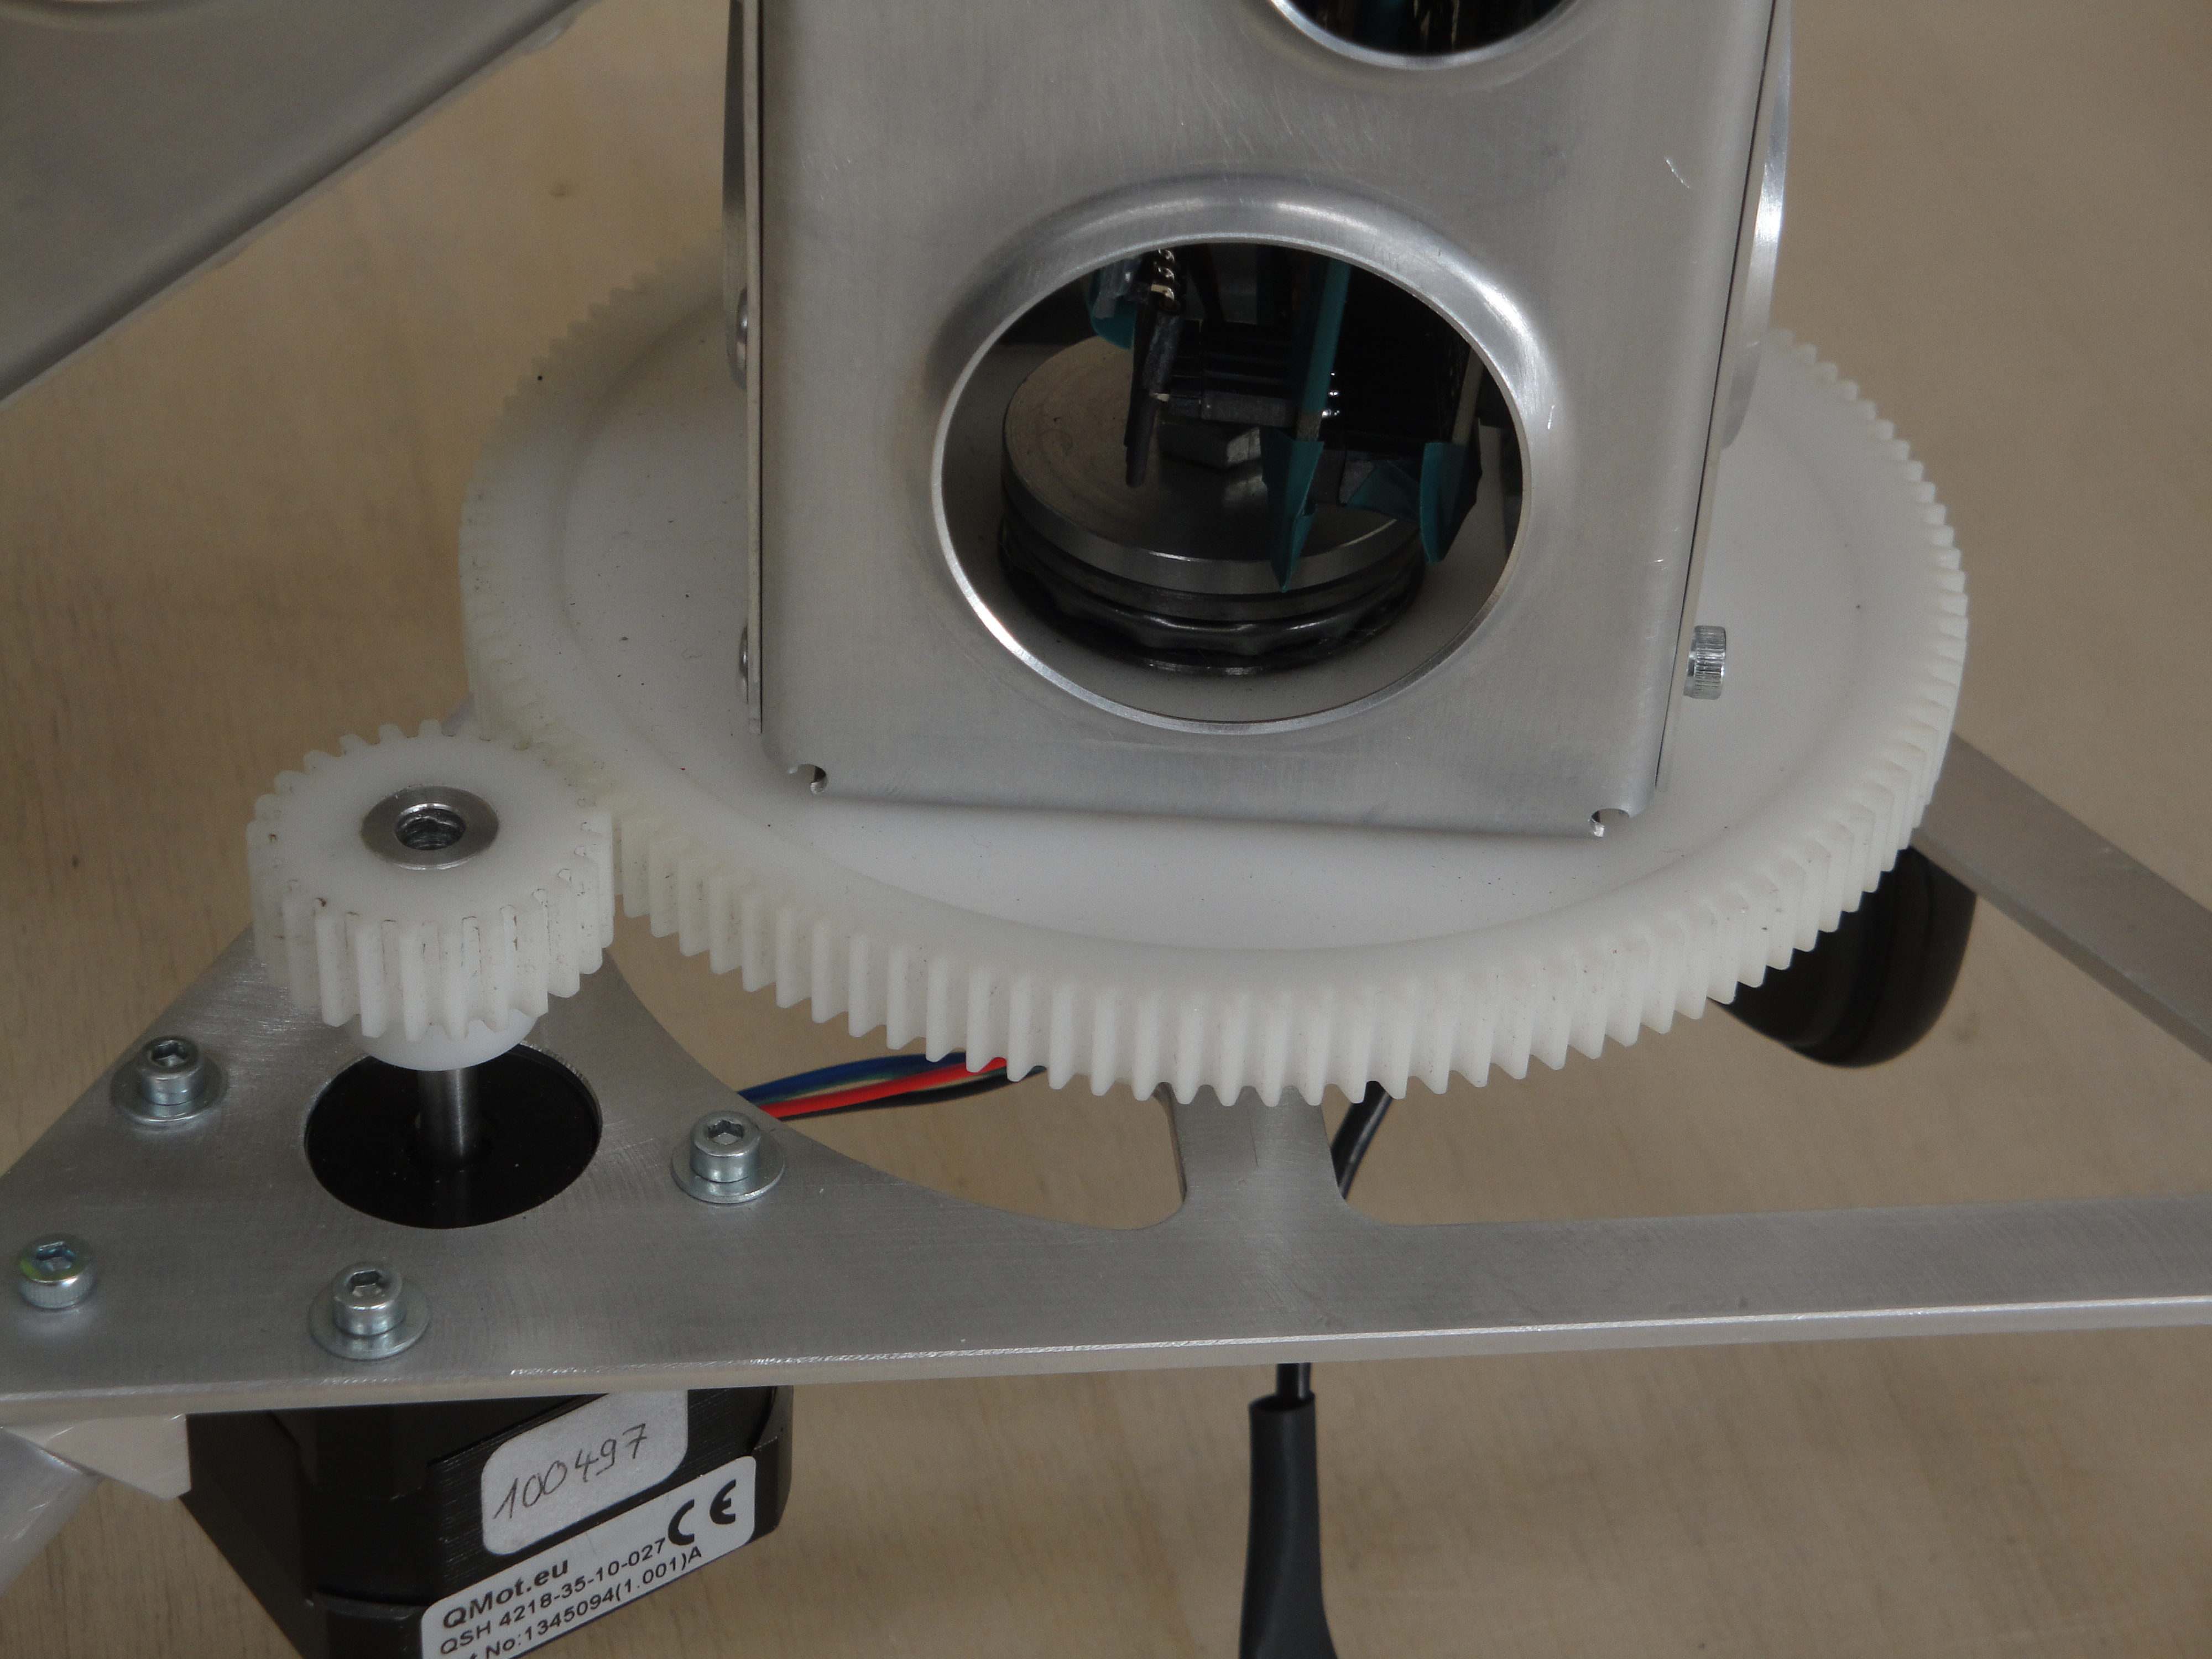
\includegraphics[width=1.0\textwidth, trim=0 0 0 0, clip=true]{../doc/fig/DSC02962.JPG}
        \end{column}
    \end{columns}
\end{frame}
\begin{frame}
    \frametitle{Turm}
    \begin{columns}
        \begin{column}{0.8\textwidth}
            \centering
            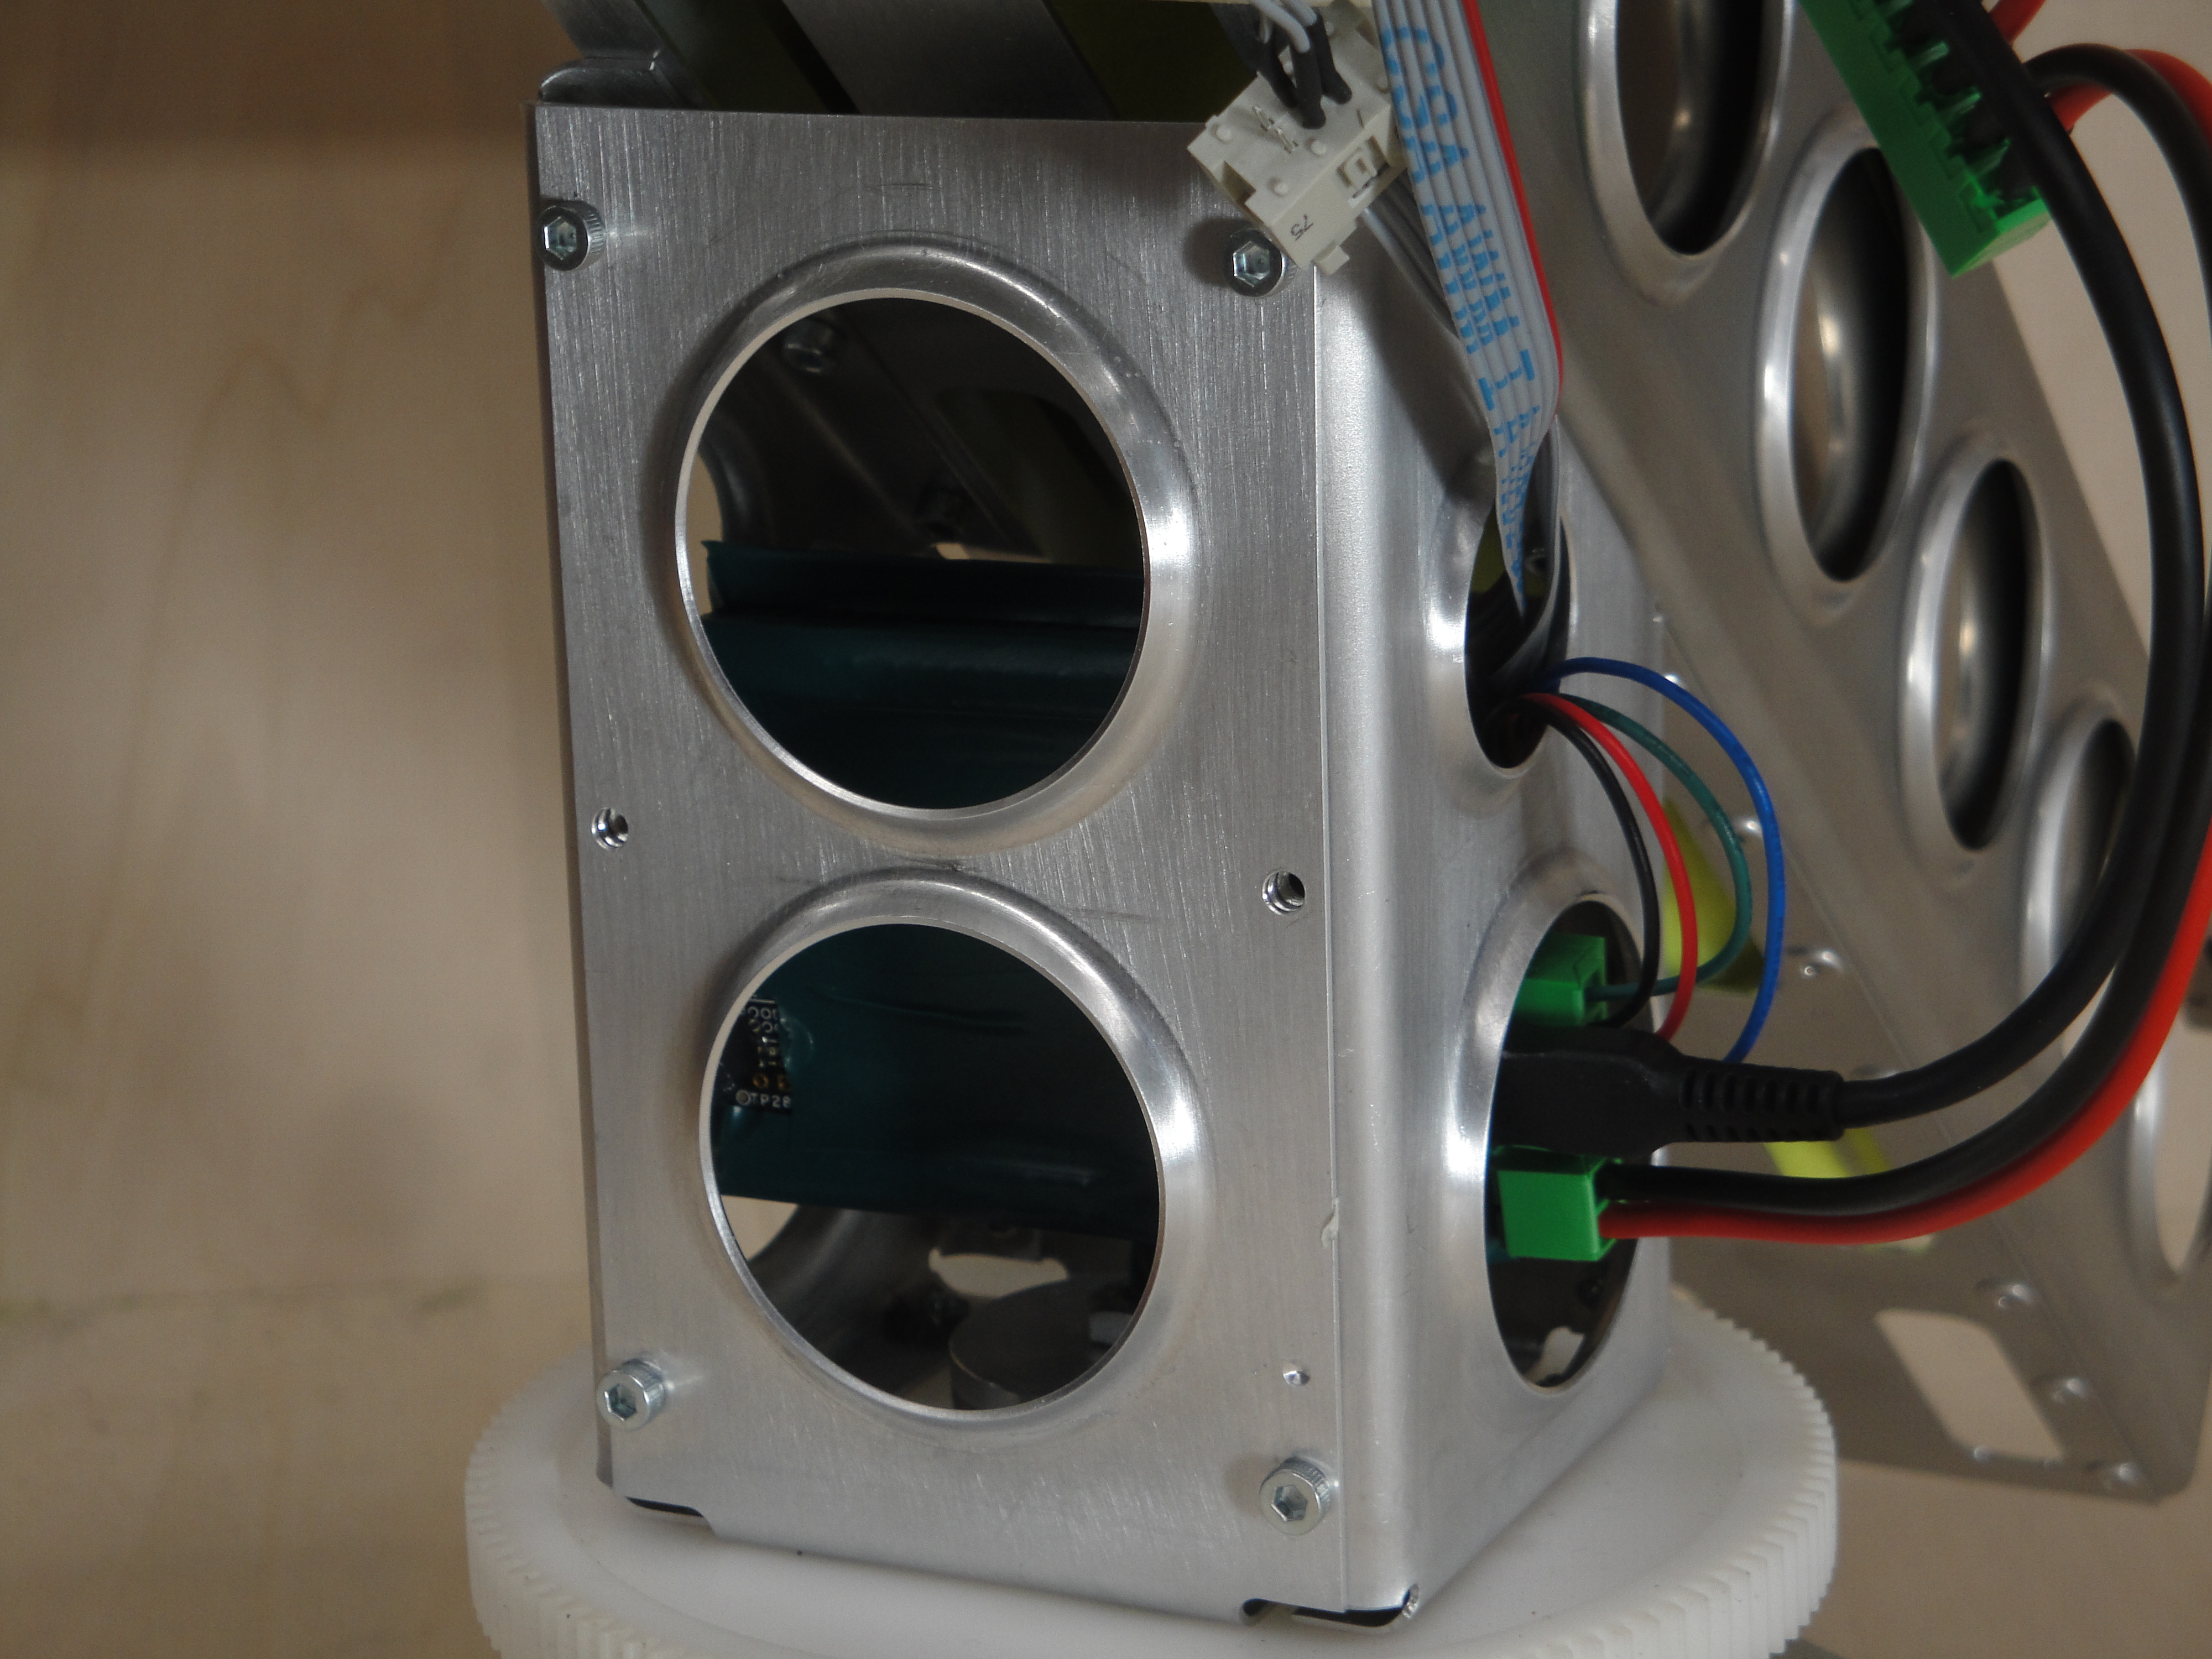
\includegraphics[width=1.0\textwidth]{../doc/fig/DSC02985.JPG}
        \end{column}
    \end{columns}
\end{frame}

\subsection{Ballbeförderung}
\begin{frame}
    \frametitle{Balllager}
    \begin{columns}
        \begin{column}{0.7\textwidth}
            \centering
            \includegraphics[width=1.0\textwidth]{FotosM/Bild7.png}
        \end{column}
    \end{columns}
\end{frame}
\begin{frame}
    \frametitle{Ballnachschub}
    \begin{columns}
        \begin{column}{0.8\textwidth}
            \centering
            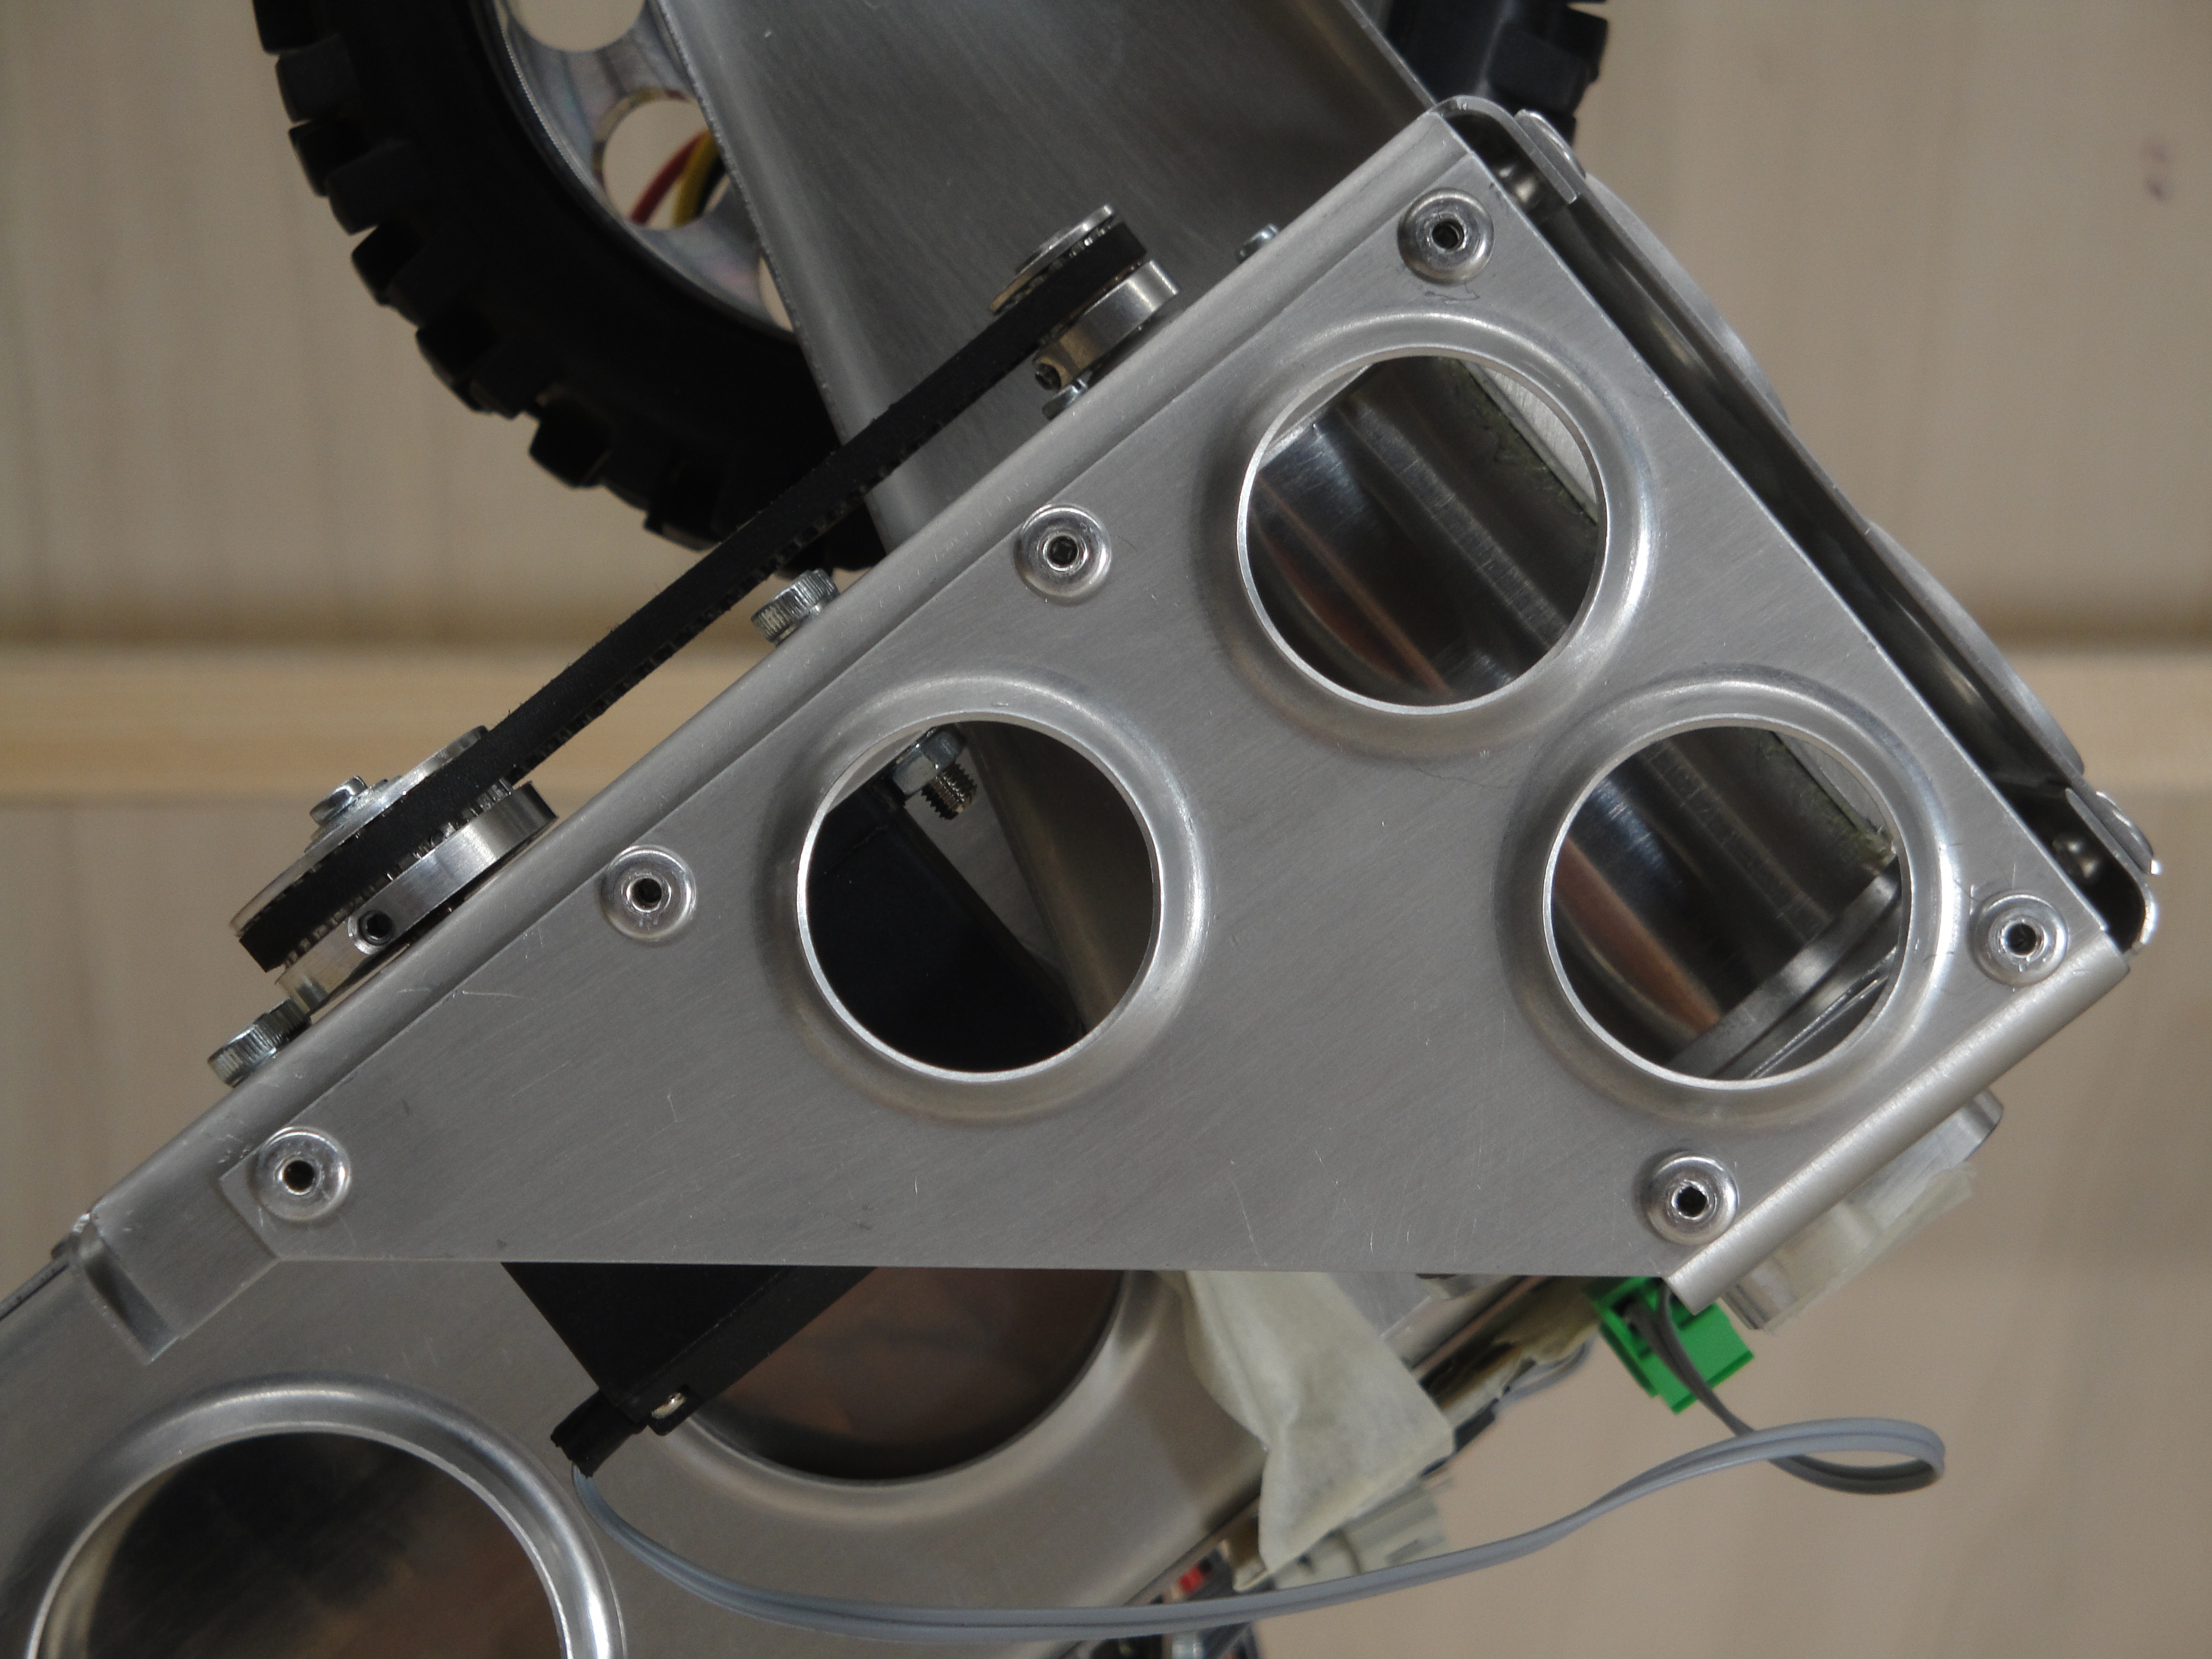
\includegraphics[width=1.0\textwidth]{../doc/fig/DSC02958.JPG}
        \end{column}
    \end{columns}
\end{frame}
\begin{frame}
    \frametitle{Ballbeförderung}
    \begin{columns}
        \begin{column}{0.8\textwidth}
            \centering
            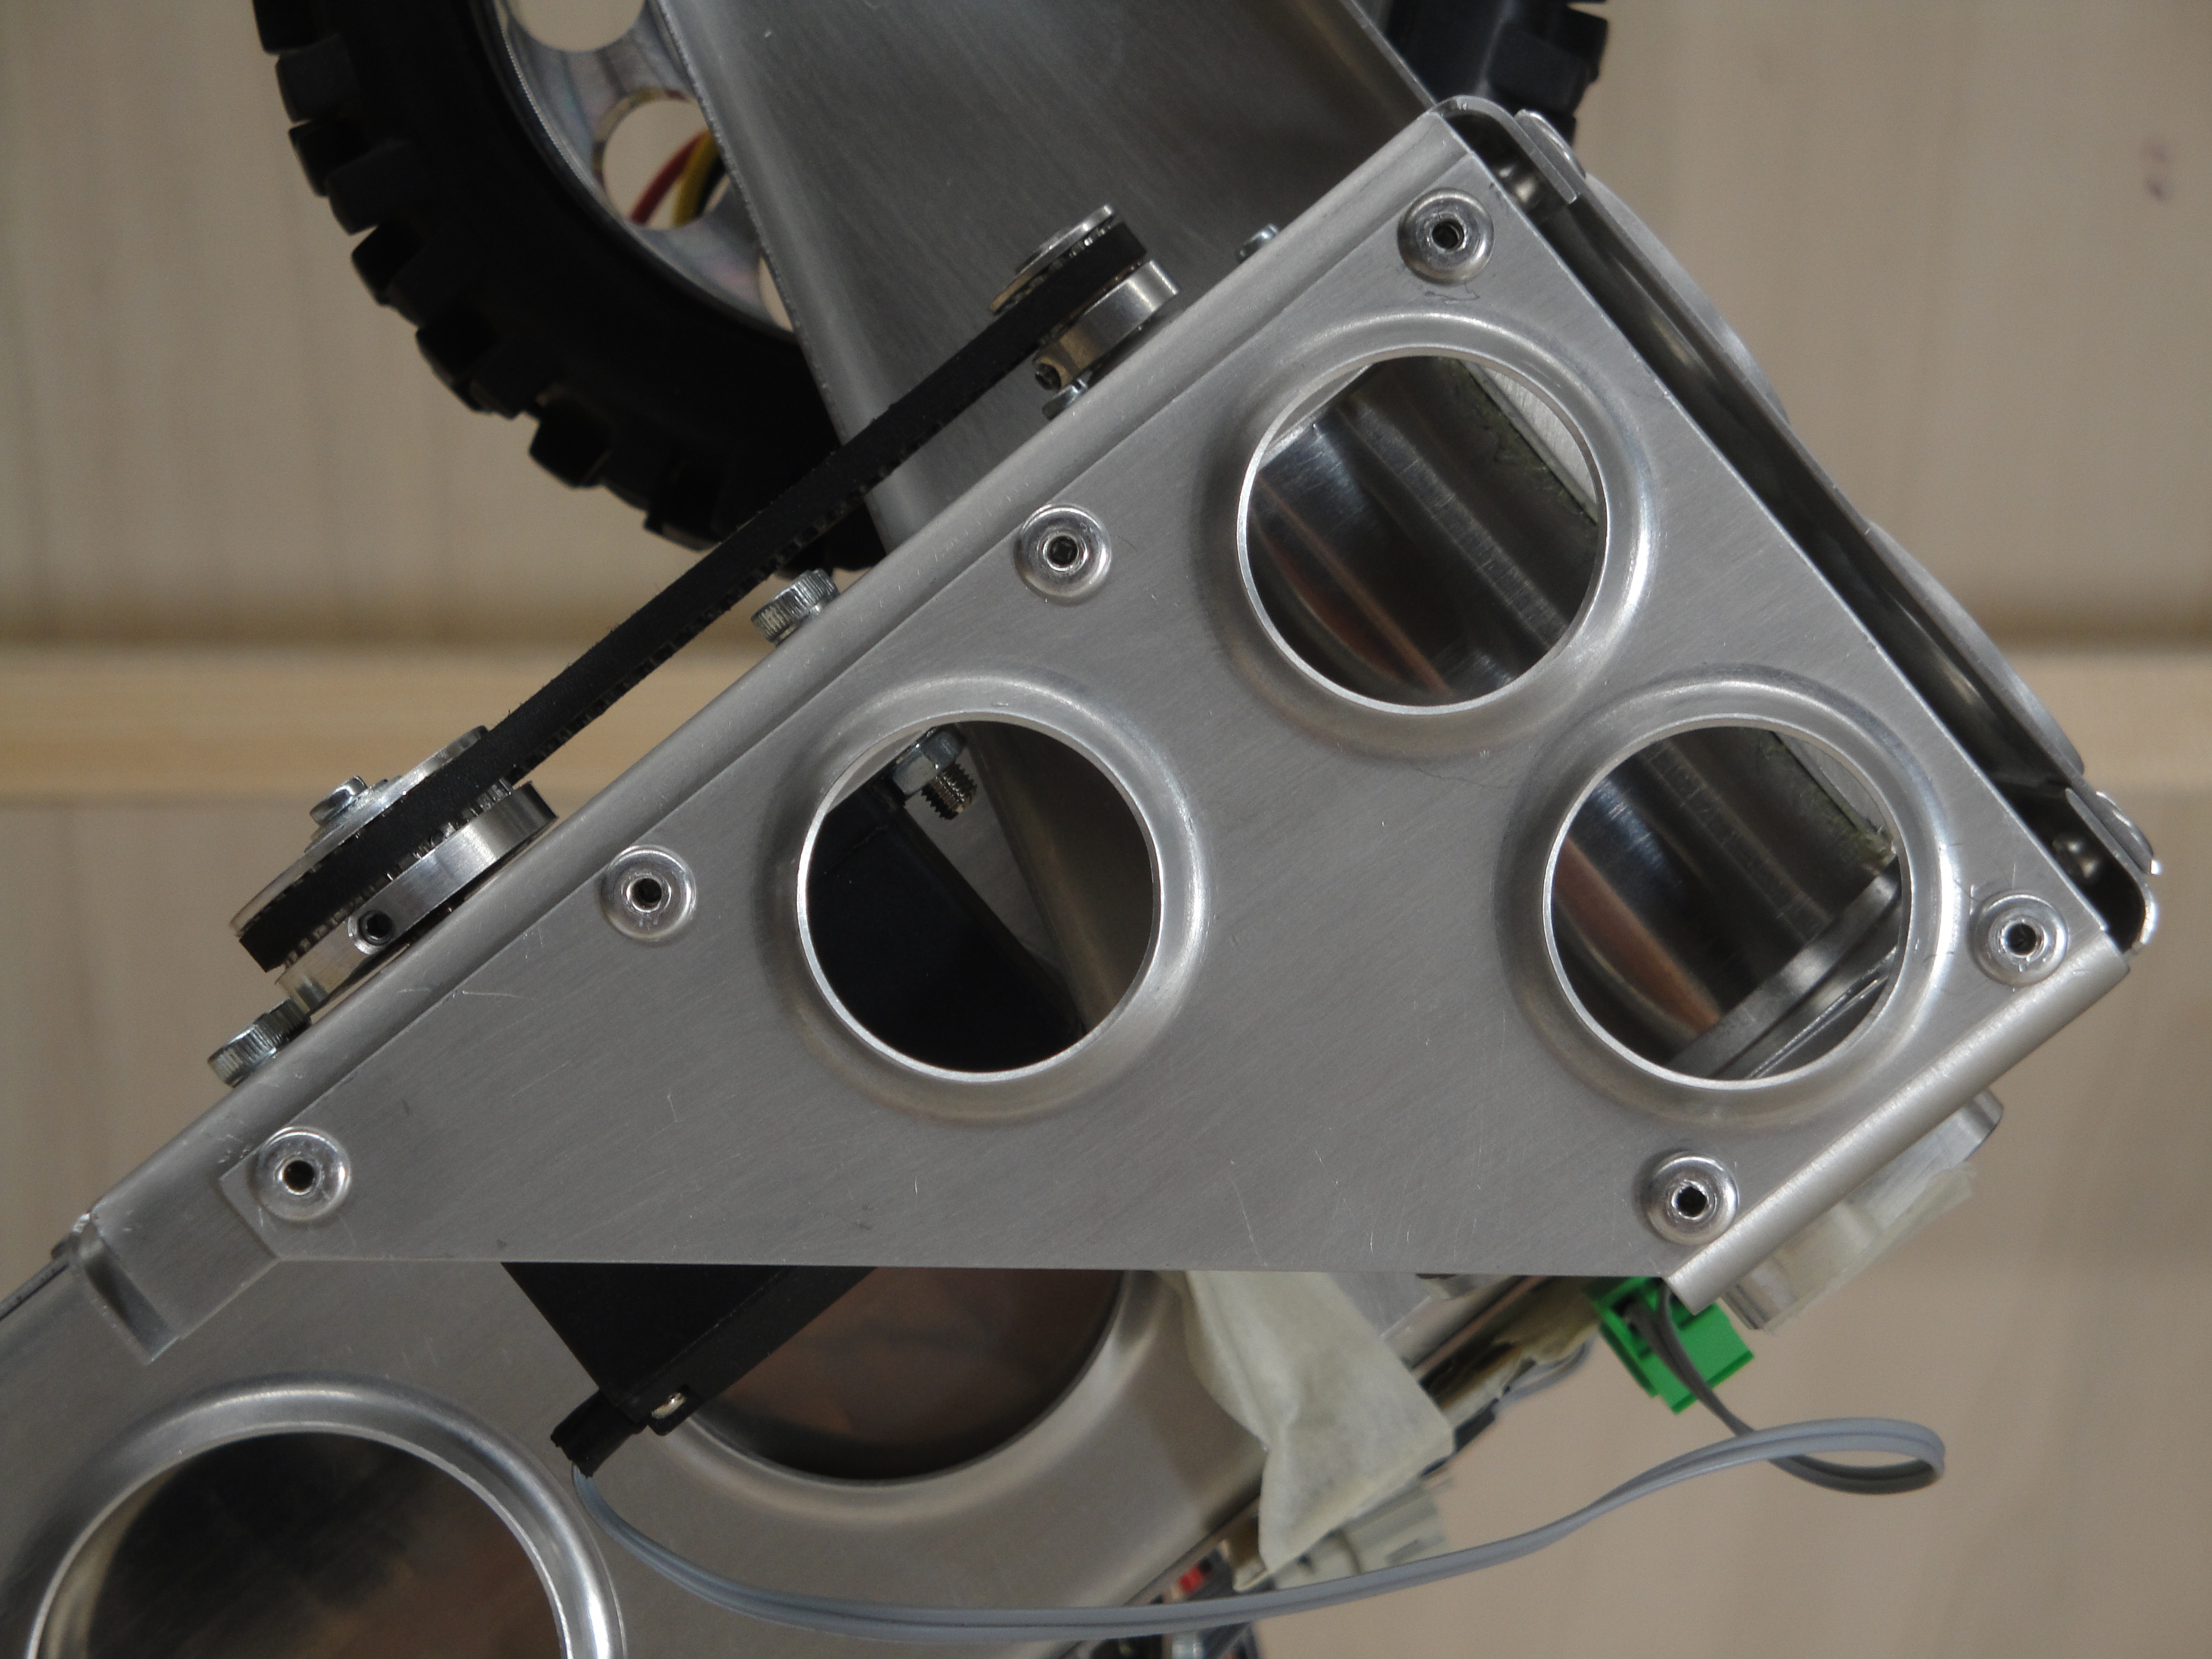
\includegraphics[width=1.0\textwidth]{../doc/fig/DSC02958.JPG}
        \end{column}
    \end{columns}
\end{frame}

\subsection{Ansteuerung BLDC Motor}
\label{sec:bldc}
Die Ansteuerung für den BLDC Motor\footnote{\textbf{B}rush\textbf{L}ess 
\textbf{D}irect \textbf{C}urrent Motor} wird in in der Gruppe PREN-ET 
entwickelt. (Siehe \ref{sec:pren-et} \nameref{sec:pren-et}) 
Daher werden hier nur Anpassungen für das Tem 27 betrachtet. 
\begin{figure}[h!]
    \centering
    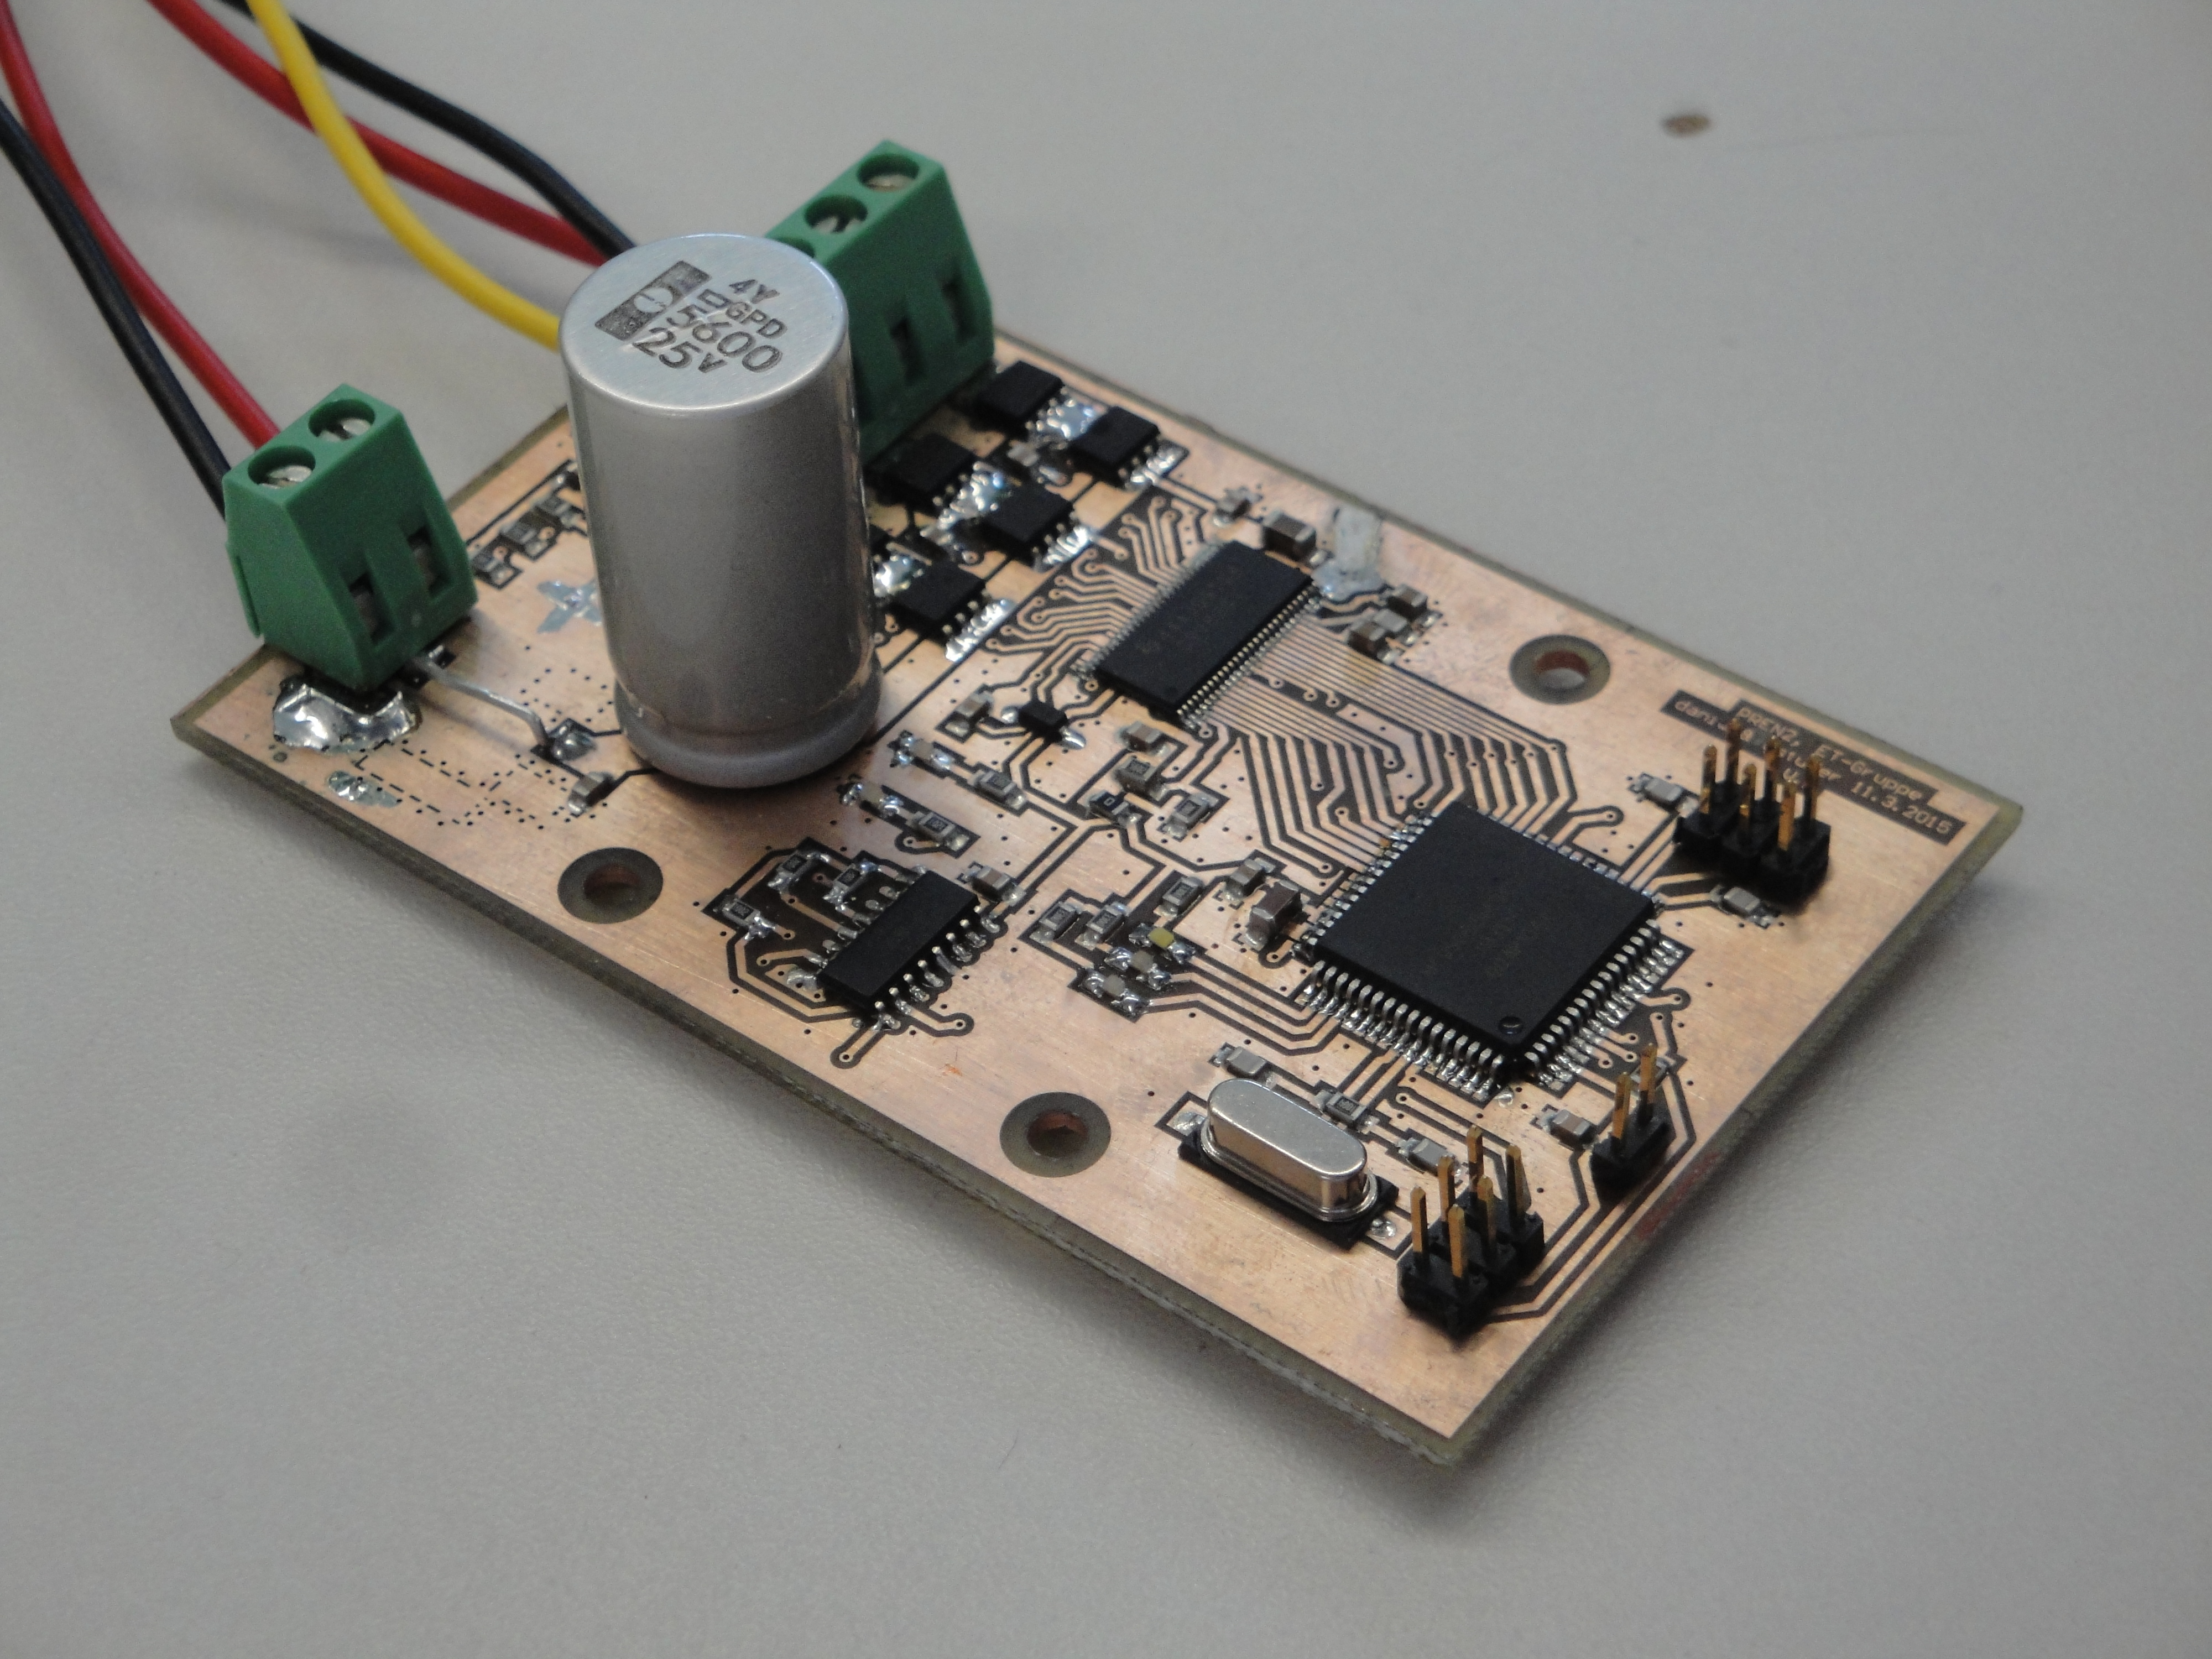
\includegraphics[width=0.7\textwidth]{fig_pcb/DSC02906.JPG}
    \caption{Ansteuerung BLDC Motor}
    \label{fig:dc}
\end{figure}

\subsection{Ansteuerung Motor Ballnachschub}
\label{sec:dc}
Die Ansteuerung für den Motor für den Ballnachschub wird in in der Gruppe 
PREN-ET entwickelt. (Siehe \ref{sec:pren-et} \nameref{sec:pren-et})
%Daher werden hier nur Anpassungen für das Team 27 betrachtet. 
\begin{figure}[h!]
    \centering
    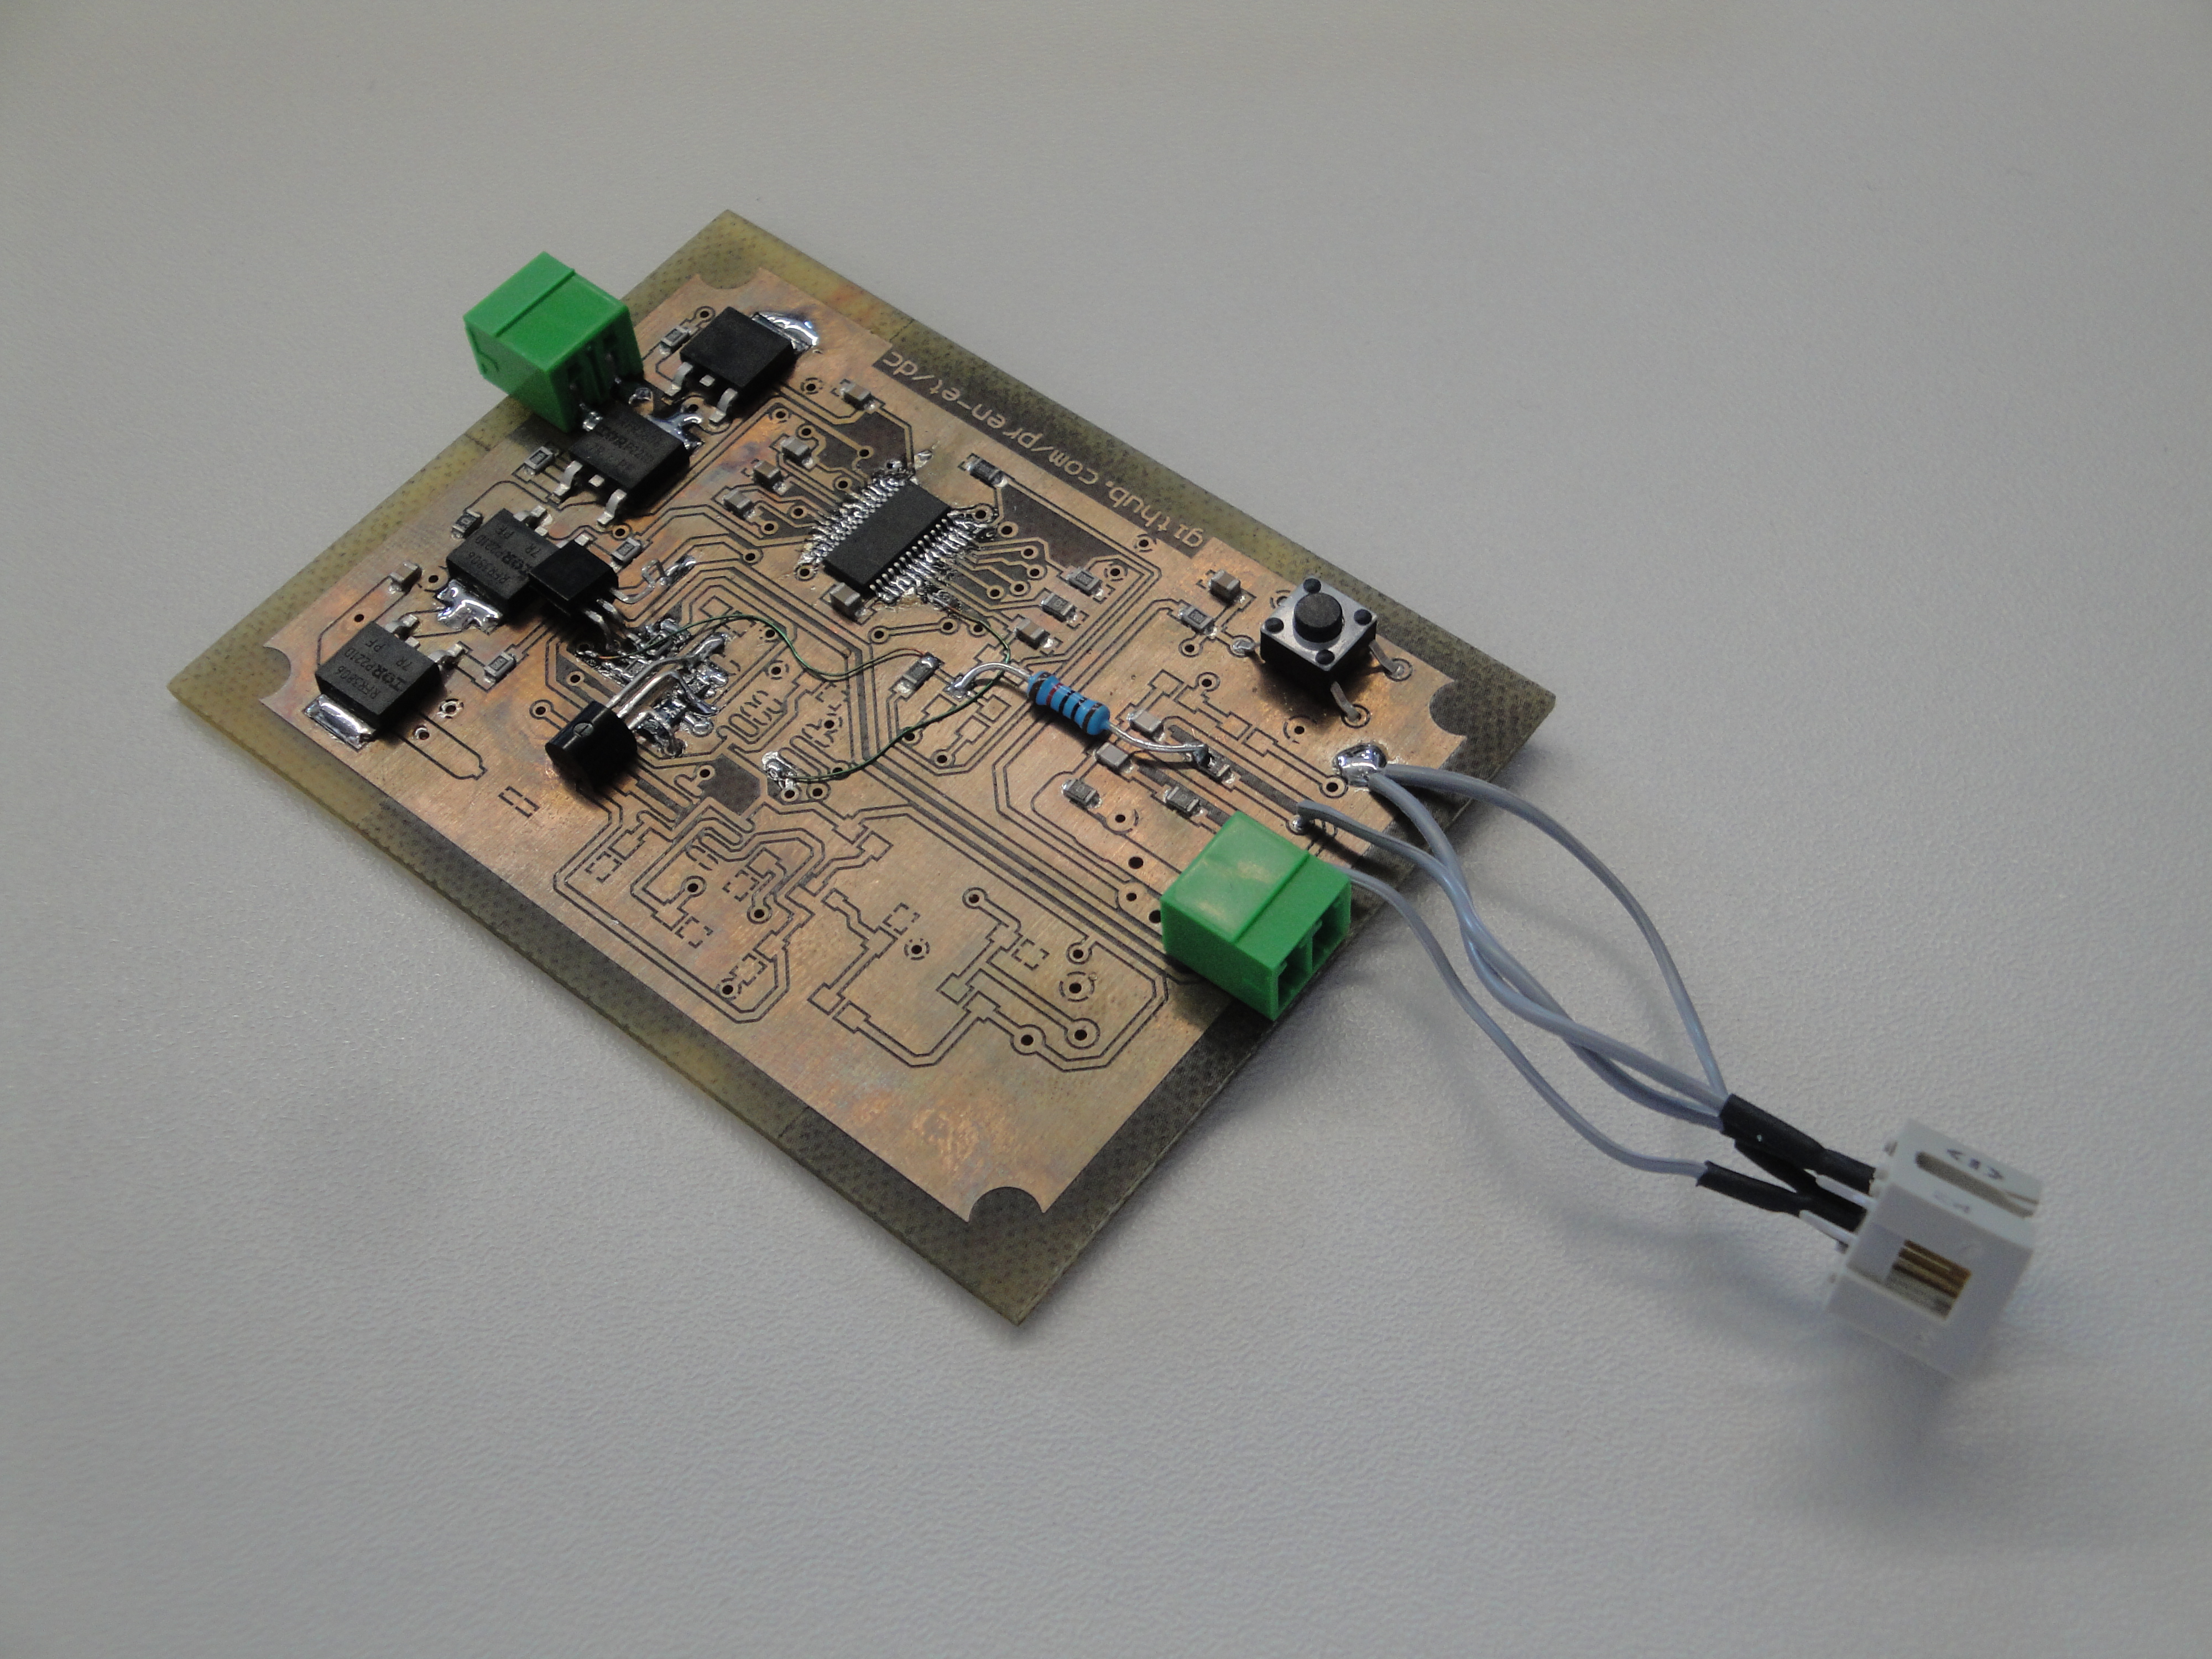
\includegraphics[width=0.7\textwidth]{fig_pcb/DSC02909.JPG}
    \caption{Ansteuerung Ballnachschub}
    \label{fig:dc}
\end{figure}

\noindent
Der Gleichstrommotor für den Ballnachschub wird mit einem 
PWM\footnote{\textbf{P}ulse \textbf{W}idth \textbf{M}odulation} Signal 
angesteuert. Über das Puls-Pausen-Verhältnis kann die Leistung des Motors 
eingestellt werden. 

\begin{frame}
    \frametitle{Energieversorgung}
    \begin{columns}
        \begin{column}{0.50\textwidth}
            \centering
            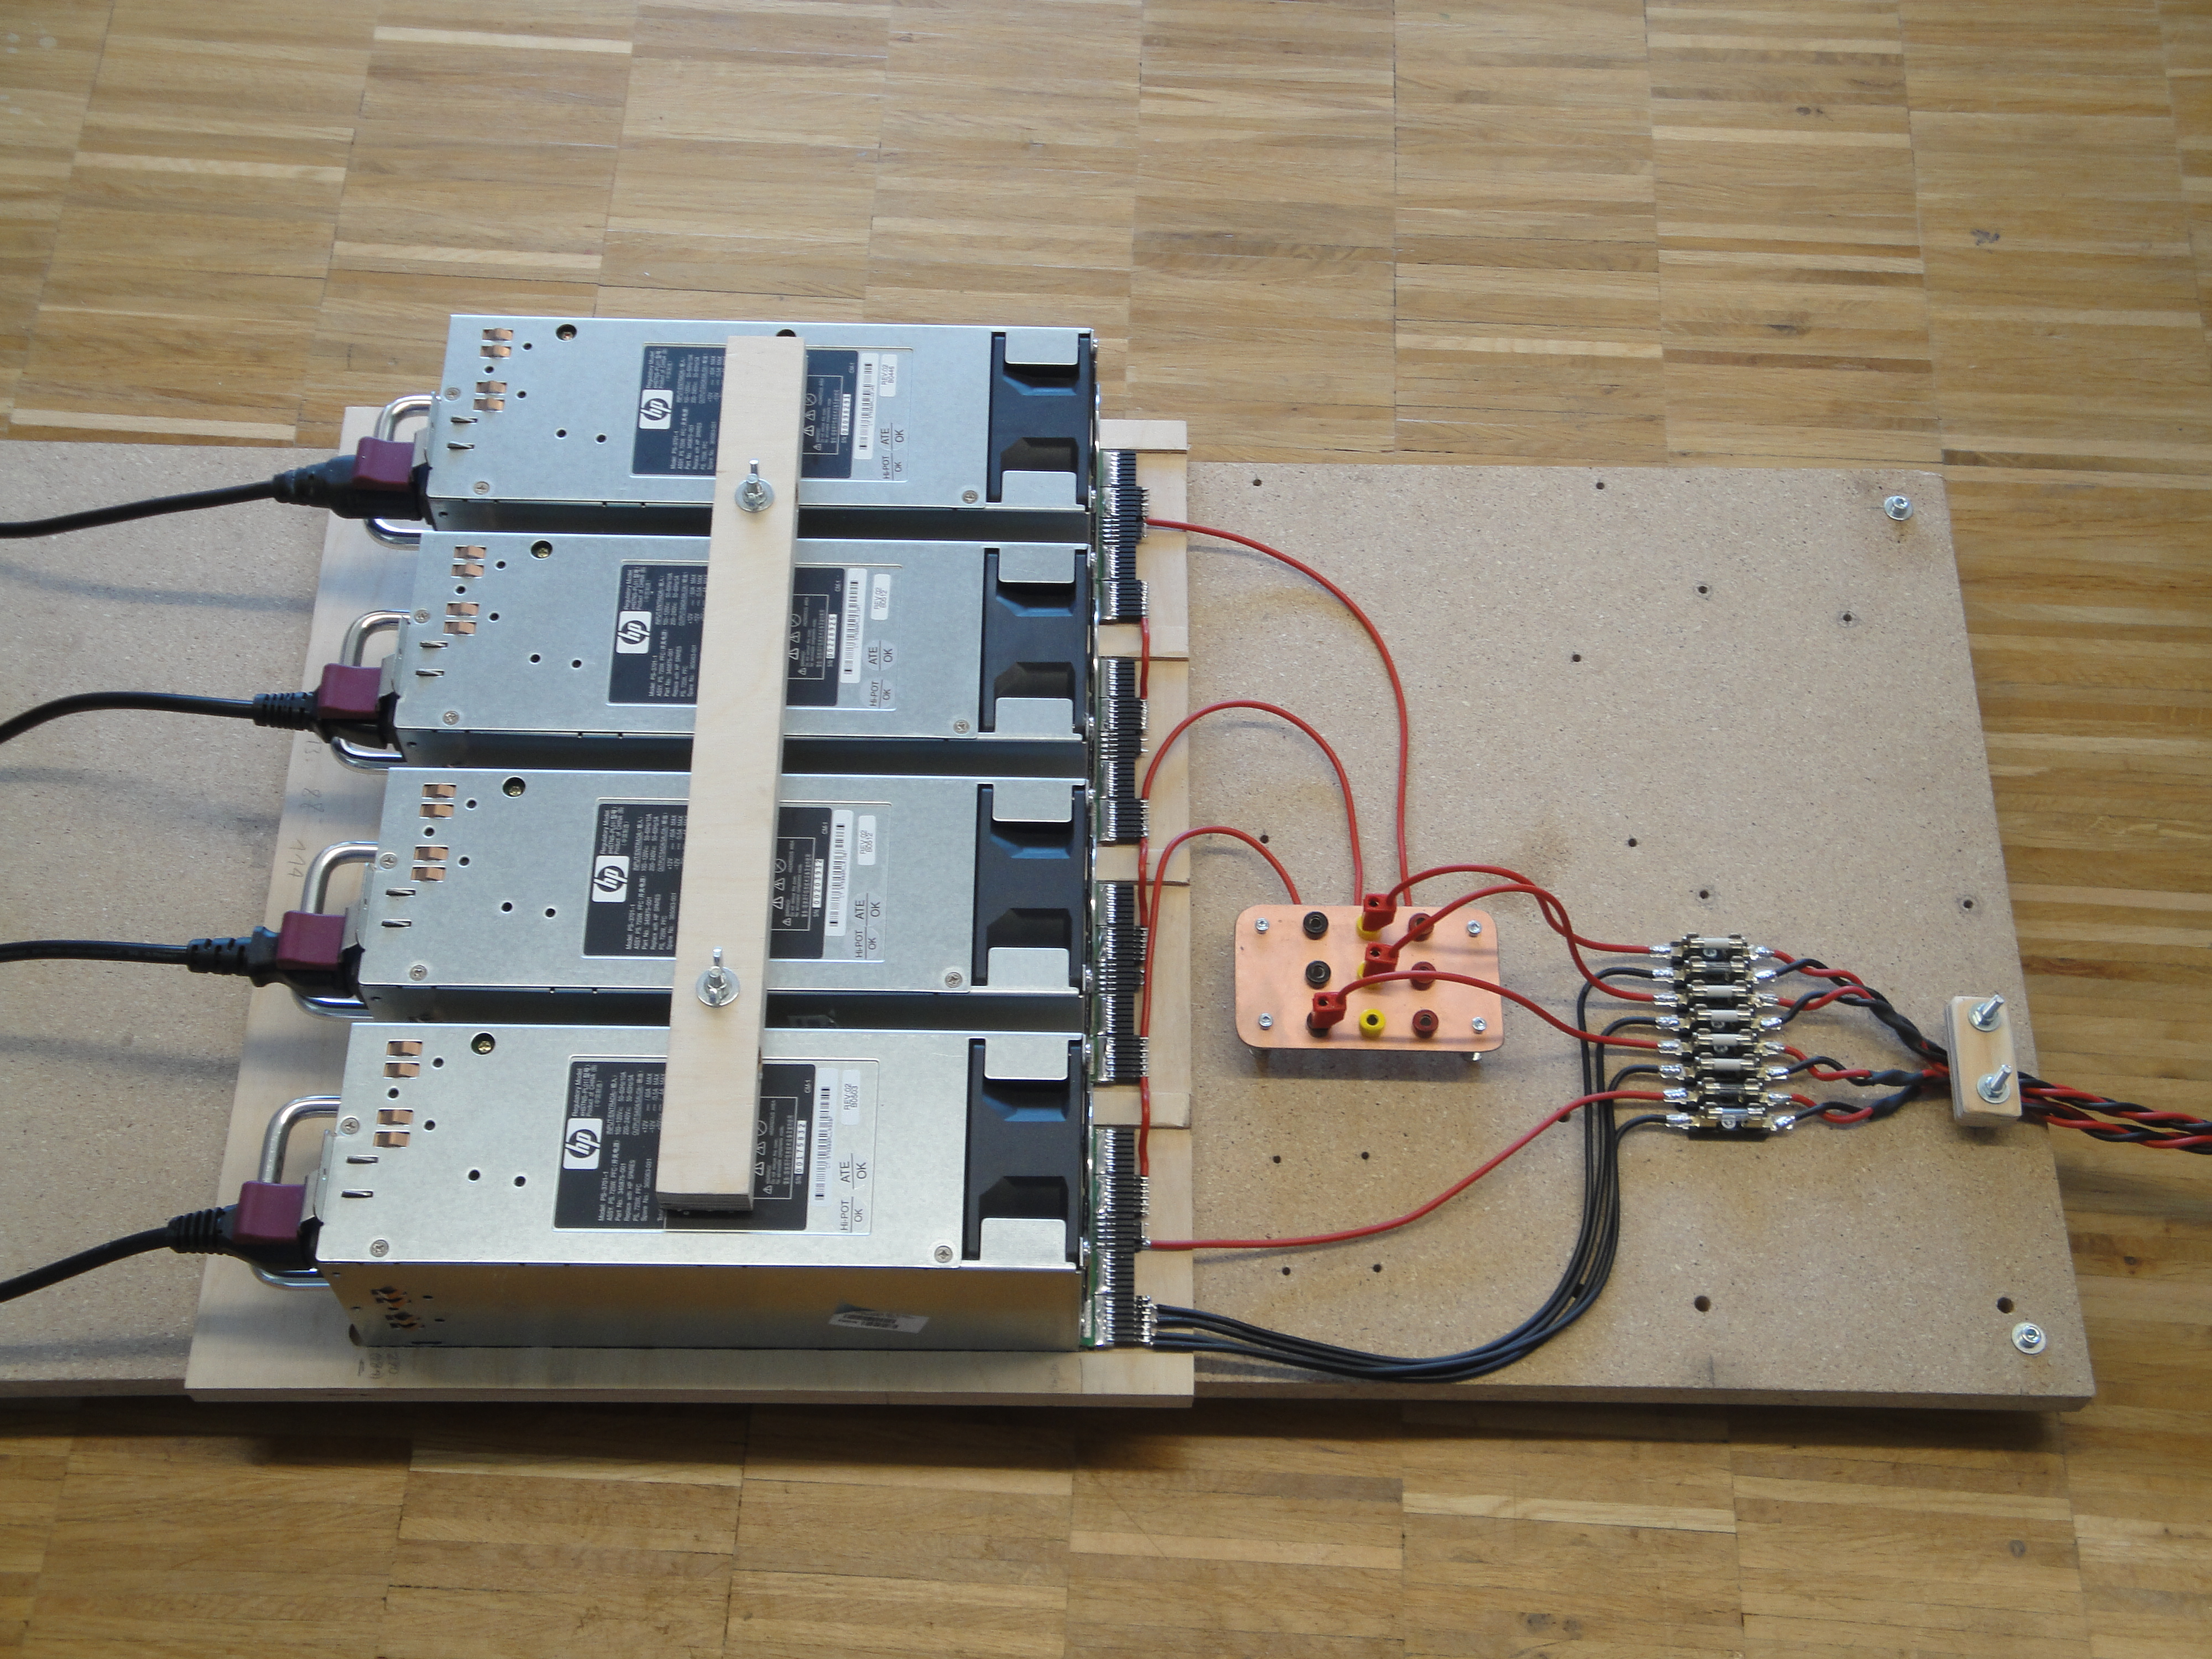
\includegraphics[width=1.00\textwidth]{../doc/fig/DSC02936.JPG}
        \end{column}
        \begin{column}{0.50\textwidth}
            \begin{block}{Netzteil}
                \begin{itemize}
                    \item Servernetzteile
                    \item Galvanische Trennung
                    \item Verschiedene Spannungen
                    \begin{tabular}{@{}l@{$~\to~$}l@{}}
                        5\si{\volt}  & Steuerung \\
                        12\si{\volt} & Gleichstrommotor \\
                        24\si{\volt} & Schrittmotor / BLDC \\
                        48\si{\volt} & - \\
                    \end{tabular}
                \end{itemize}
            \end{block}
        \end{column}
    \end{columns}
\end{frame}

\begin{frame}
    \frametitle{Ablauf}
    \begin{columns}
        \begin{column}{1\textwidth}
            \centering
            \includegraphics[width=1.0\textwidth]{../doc/fig/Sequenzdiagramm.png}
        \end{column}
    \end{columns}
\end{frame}


\section{Kenndaten}
\begin{frame}
    \begin{columns}
        \begin{column}{0.50\textwidth}
            \centering
            \includegraphics[width=1.00\textwidth]{../doc/fig/Bild_mit_Kamera.png}
        \end{column}
        \begin{column}{0.50\textwidth}
            \begin{block}{Kenndaten Twentyseven}
                \begin{itemize}
                    \item Gewicht 1932\si{\gram}
                    \item Zeit: 3\si{\second}
                    \item Treffsicherheit: 5/5
                \end{itemize}
            \end{block}
        \end{column}
    \end{columns}
\end{frame}

\section{Rückblick - Ausblick} % Peter
\begin{frame}
    \begin{block}{So wars - So wirds}
        \begin{itemize}
            \item Team
            \begin{itemize}
                \item Harmonie
                \item Ambitioniert
                \item Zielorientiert
            \end{itemize}
            \item Aufgabe
            \begin{itemize}
                \item Vielfalt
            \end{itemize}
            \item Wettbewerb
            \begin{itemize}
                \item Optimistisch
                \item Top 5
            \end{itemize}
        \end{itemize}
    \end{block}
\end{frame}

